

\chapter{PENGUJIAN DAN ANALISIS}
\label{chap:pengujiananalisis}

Pada bab ini, akan dibahas mengenai pengujian sistem yang telah dikembangkan,
termasuk skenario pengujian yang dilakukan, hasil pengujian, serta analisis
terhadap performa sistem. Pengujian ini bertujuan untuk memastikan bahwa sistem berfungsi
sesuai dengan spesifikasi yang telah ditetapkan dan dapat memenuhi kebutuhan pengguna.

\section{\emph{Unit Testing}}
Pengujian unit bertujuan untuk memastikan bahwa setiap bagian sistem, baik
perangkat keras maupun perangkat lunak, berfungsi dengan baik dan sesuai dengan spesifikasinya.
Pengujian ini mencakup verifikasi sistem kelistrikan serta pengujian masing-masing
submodul perangkat lunak. Adapun skenario pengujian yang dilakukan dijelaskan sebagai
berikut.

\subsection{Pengujian Sistem Elektrikal}
Pengujian sistem elektrikal bertujuan untuk memastikan bahwa seluruh komponen perangkat
keras beroperasi dengan baik dan sesuai dengan spesifikasi teknis yang telah ditetapkan.
Pengujian ini meliputi pengukuran tegangan, verifikasi koneksi, serta uji
fungsionalitas tiap komponen. Pengukuran tegangan dilakukan menggunakan osiloskop
guna memastikan bahwa tegangan yang diterima oleh setiap komponen berada dalam batas
toleransi yang diizinkan. Dikarenakan semua komponen perangkat keras menggunakan
catu daya yang sama maka pengujian hanya dilakukan pada satu titik tegangan, yaitu
pada tegangan 24VDC. Adapun gambar pengujian sebagai berikut:

\begin{figure}[H]
	\centering
	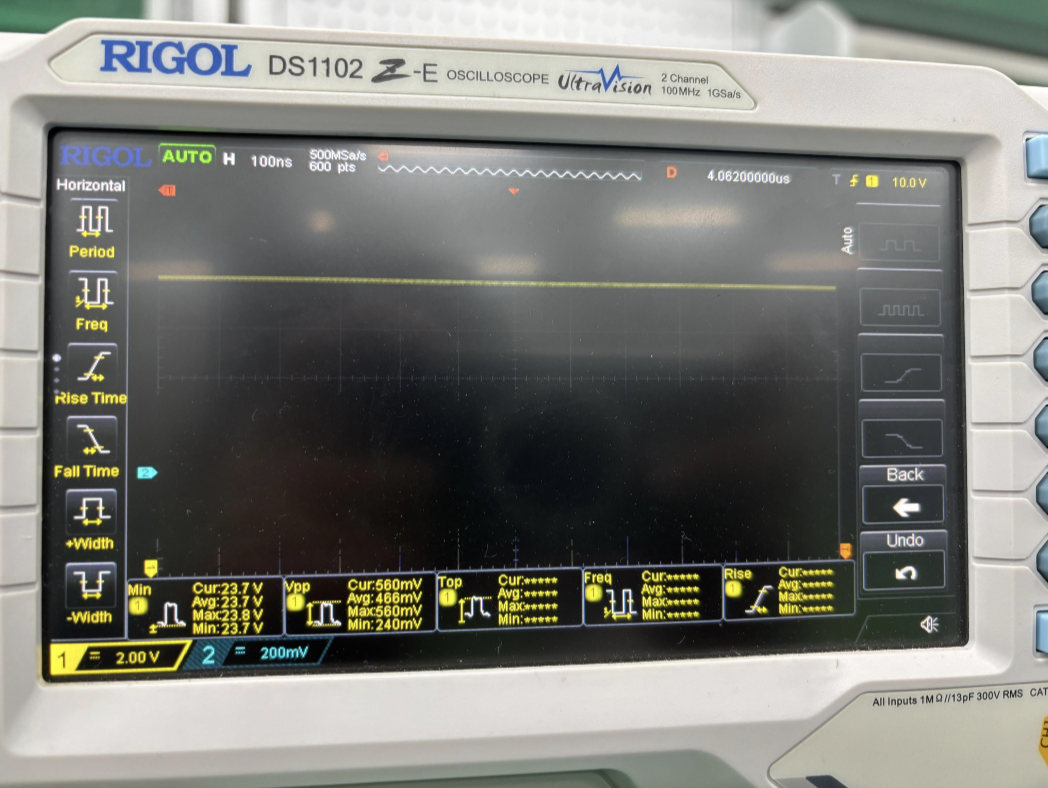
\includegraphics[scale=0.5]{gambar/bab4/osii.png}
	\caption{Pengujian Tegangan 24V dengan osiloskop}
	\label{fig:pengujian_tegangan} \footnotesize{\textbf{Sumber:} Dokumentasi Penulis}
\end{figure}

Berdasarkan pengukuran tegangan yang dilakukan, dimana teggangan akan direkam
dalam 5 yang dilakukan sebanyak 10 kali pengulangan, maka didapatkan hasil yang dapat
dilihat pada tabel \ref{tab:pengujian_tegangan}
\begin{table}[H]
	\centering
	\caption{Hasil Pengujian Tegangan 24VDC pada Sistem Elektrikal}
	\label{tab:pengujian_tegangan}
	\begin{tabular}{|c|c|c|c|l|l|}
		\hline
		\textbf{Ke-} & \textbf{Min (V)} & \textbf{Maks (V)} & \textbf{Avg (V)} & \textbf{Kondisi} & \textbf{Keterangan}      \\
		\hline
		1            & 24.0             & 24.0              & 24.0             & Belum terpasang  & Tegangan sangat stabil   \\
		2            & 23.8             & 23.9              & 23.9             & Belum terpasang  & Tanpa beban              \\
		3            & 23.7             & 23.9              & 23.8             & Idle             & Tegangan stabil          \\
		4            & 23.4             & 23.7              & 23.6             & PTZ bergerak     & Drop saat motor aktif    \\
		5            & 23.7             & 23.9              & 23.8             & Idle             & Normal                   \\
		6            & 23.8             & 23.9              & 23.8             & Idle             & Stabil                   \\
		7            & 23.4             & 23.8              & 23.6             & PTZ bergerak     & Tegangan drop saat gerak \\
		8            & 23.7             & 23.9              & 23.8             & Idle             & Stabil                   \\
		9            & 23.7             & 23.8              & 23.7             & Idle             & Stabil                   \\
		10           & 23.7             & 23.9              & 23.8             & Idle             & Normal                   \\
		\hline
	\end{tabular}
\end{table}

Hasil pengujian menunjukkan bahwa tegangan 24VDC pada sistem elektrikal stabil
dan sesuai dengan spesifikasi yang diharapkan. Tegangan tetap berada dalam rentang
yang aman untuk semua komponen, meskipun terjadi sedikit penurunan saat motor
PTZ bergerak. Penurunan ini masih dalam batas toleransi yang dapat diterima,
sehingga tidak mempengaruhi kinerja sistem secara keseluruhan.

\begin{table}[H]
	\centering
	\caption{Perhitungan Rata-rata Tegangan dan Error dari Ideal 24.0V}
	\label{tab:rata_rata_error}
	\begin{tabular}{|l|c|c|}
		\hline
		\textbf{Jenis Tegangan} & \textbf{Rata-rata (V)} & \textbf{Error dari 24.0V (V)} \\
		\hline
		Minimum                 & 23.73                  & 0.27                          \\
		Maksimum                & 23.87                  & 0.13                          \\
		Rata-rata (Avg)         & 23.82                  & 0.18                          \\
		\hline
	\end{tabular}
\end{table}

Rata-rata tegangan minimum yang tercatat selama pengujian adalah sebesar 23{,}73
V, dengan deviasi maksimum terhadap nilai ideal 24,0 V sebesar 0{,}27 V. Nilai ini
menunjukkan bahwa meskipun terjadi penurunan tegangan, sistem masih berada dalam
batas toleransi yang aman. Sementara itu, rata-rata tegangan maksimum berada
pada 23{,}87 V, yang mengindikasikan bahwa sistem beroperasi secara stabil tanpa
melebihi batas suplai yang ditentukan. Secara keseluruhan, rata-rata tegangan selama
pengujian adalah 23{,}82 V, dengan error sebesar 0{,}18 V terhadap nilai ideal. Nilai
ini masih tergolong kecil dan tidak memberikan dampak signifikan terhadap performa
sistem elektrikal 24 VDC. Hal ini menunjukkan bahwa sistem distribusi daya
bekerja dengan stabil dan toleransi tegangan masih berada dalam rentang aman
untuk pengoperasian seluruh perangkat keras.

Pengujian koneksi dilakukan dengan memanfaatkan perintah \emph{ping} dan \emph{traceroute}
untuk memastikan bahwa tidak terdapat sambungan yang terputus maupun kesalahan
koneksi antar komponen. Selanjutnya, pengujian fungsionalitas dilakukan dengan
menjalankan masing-masing komponen secara independen untuk memverifikasi bahwa
setiap modul dapat beroperasi sesuai dengan peran dan spesifikasi yang telah
ditentukan. Pengujian konektivitas jaringan dilakukan untuk memastikan bahwa seluruh
perangkat yang tergabung dalam sistem dapat saling terhubung melalui jaringan lokal.
Pengujian dilakukan menggunakan perintah \textit{ping} dari dua sisi utama,
yaitu dari komputer pada robot dan dari komputer pada \textit{control station}.
Tujuan pengujian ini adalah untuk memverifikasi keterhubungan antar perangkat
serta memastikan latensi (delay) komunikasi berada dalam rentang yang rendah dan
dapat diterima. Pengujian konektivitas dilakukan dengan mengirimkan perintah \textit{ping}
sebanyak 10 kali ke setiap perangkat dalam jaringan, baik dari komputer pada robot
maupun dari komputer \textit{control station}. Berdasarkan hasil pengujian,
seluruh perangkat merespons dengan baik tanpa adanya \textit{packet loss}. Rata-rata
delay atau waktu tunda (\textit{round-trip time}) yang tercatat berada dalam kisaran
1{,}2 ms hingga 4{,}7 ms, tergantung pada posisi dan jenis perangkat yang diuji.
Adapun rata-rata delay dari beberapa perangkat kunci adalah sebagai berikut:
koneksi dari komputer \textit{control station} ke kamera thermal memiliki rata-rata
delay sebesar 2{,}5 ms, ke komputer robot sebesar 3{,}1 ms, dan ke router station
sebesar 1{,}8 ms. Sementara dari sisi robot, \textit{ping} ke kamera thermal
menunjukkan rata-rata delay sebesar 3{,}3 ms, sedangkan ke \textit{control
station} sebesar 3{,}0 ms. Secara keseluruhan, nilai rata-rata delay dari
seluruh pengujian berada pada 2{,}77 ms, yang masih tergolong sangat kecil dan memenuhi
syarat untuk sistem komunikasi waktu nyata. Hasil ini menegaskan bahwa jaringan
yang digunakan cukup andal untuk menunjang proses pertukaran data dan kontrol
antar komponen sistem secara simultan dan stabil.

\subsection{Pengujian \emph{IO Package}}
Pengujian perangkat lunak IO Package bertujuan untuk memastikan bahwa semua
modul perangkat lunak yang berhubungan dengan input/output berfungsi dengan baik.
Pengujian ini mencakup pengujian RTSP Client dan PTZ Control. Pengujian RTSP
Client dilakukan untuk memastikan bahwa robot dapat menerima data video secara
real-time dari kamera thermal yang terpasang. Pengujian PTZ Control dilakukan untuk
memastikan bahwa robot dapat mengontrol orientasi kamera dengan mengunakan action.
Pengujian perangkat lunak IO Package mencakup pengujian RTSP Client dan PTZ
Control. Pada pengujian RTSP Client, dilakukan verifikasi apakah robot dapat
menerima data video secara real-time dari kamera thermal yang terpasang. Pengujian
ini dilakukan dengan memeriksa apakah aliran video dapat diterima. Hasil
pengujian menunjukkan bahwa RTSP Client berfungsi dengan baik seperti pada
Gambar \ref{fig:rtsp_client}.

\begin{figure}[H]
	\centering
	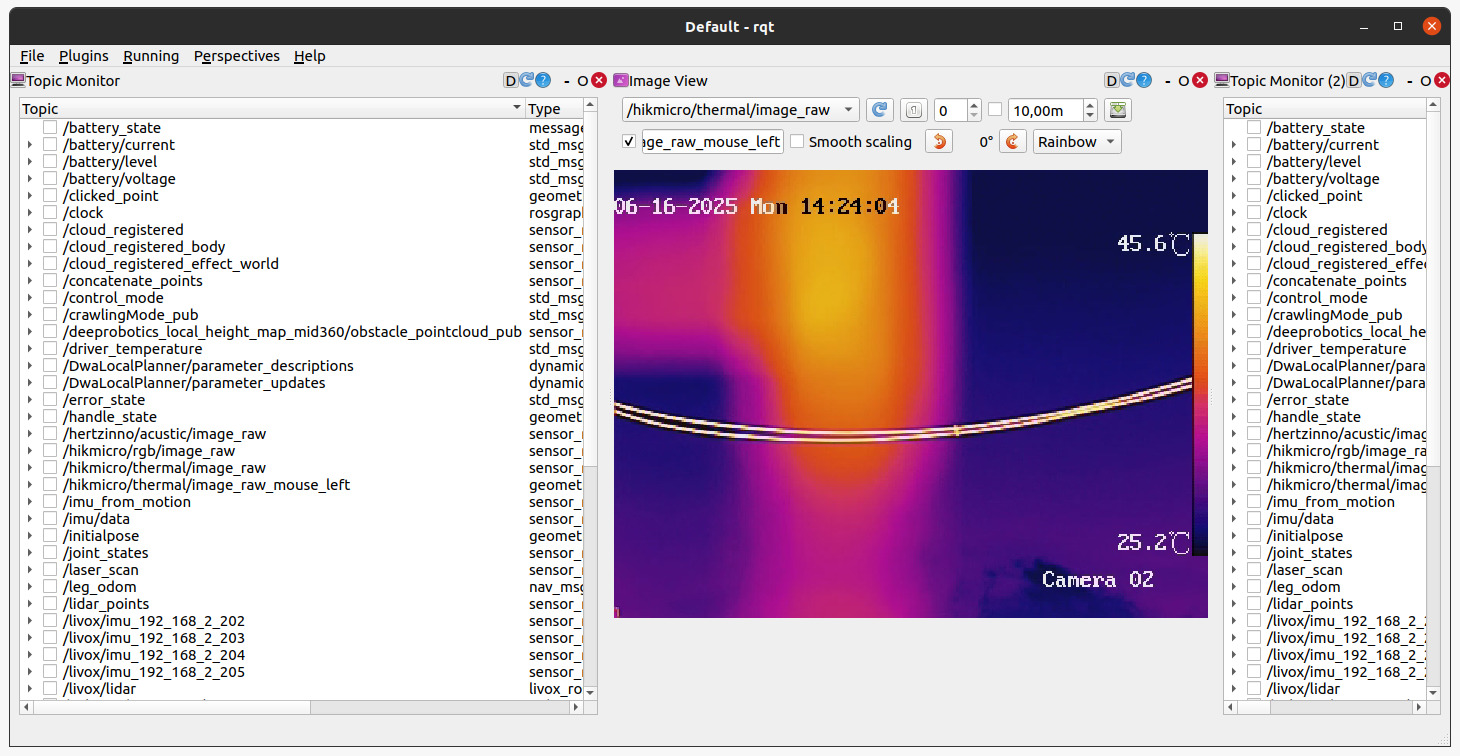
\includegraphics[width=0.9\textwidth]{gambar/bab4/test_rtsp.jpeg}
	\caption{Tampilan RQT GUI dalam Pengujian RTSP Client}
	\label{fig:rtsp_client} \footnotesize{\textbf{Sumber:} Dokumentasi Penulis}
\end{figure}

Selanjutnya pada pengujian PTZ Control, dilakukan verifikasi apakah robot dapat
mengontrol orientasi kamera dengan mengirimkan perintah \emph{pan} dan \emph{tilt}.
Sistem dianggap berhasil mencapai posisi target apabila masing-masing sumbu berada
dalam toleransi sebesar ±2 derajat dari nilai target. Pendekatan ini digunakan
untuk menghindari kondisi di mana salah satu sumbu telah stabil namun sistem
masih terus melakukan koreksi kecil terhadap sumbu lainnya yang sudah mendekati
target. Dengan demikian, waktu pencapaian dihitung sejak perintah dikirim hingga
kedua sumbu masuk ke dalam batas toleransi tersebut.

\begin{table}[H]
	\centering
	\caption{Hasil Pengujian Kontrol PID PTZ dengan Toleransi ±2°}
	\label{tab:pengujian_ptz_dual}
	\begin{tabular}{|c|c|c|c|c|c|}
		\hline
		\textbf{No} & \textbf{Target Pan (°)} & \textbf{Target Tilt (°)} & \textbf{Akhir Pan (°)} & \textbf{Akhir Tilt (°)} & \textbf{Waktu (s)} \\
		\hline
		1           & 90                      & 30                       & 89{,}5                 & 29{,}6                  & 3{,}2              \\
		2           & 180                     & -45                      & 179{,}6                & -44{,}7                 & 4{,}1              \\
		3           & 270                     & 60                       & 269{,}3                & 59{,}5                  & 12{,}2             \\
		4           & -90                     & -30                      & -89{,}5                & -29{,}6                 & 3{,}7              \\
		5           & 45                      & 15                       & 44{,}8                 & 14{,}5                  & 10{,}8             \\
		6           & 135                     & -15                      & 134{,}2                & -14{,}6                 & 3{,}6              \\
		7           & -135                    & 45                       & -134{,}4               & 44{,}3                  & 4{,}0              \\
		8           & -180                    & 60                       & -179{,}0               & 59{,}2                  & 4{,}8              \\
		9           & 60                      & 10                       & 60{,}0                 & 7{,}5                   & 11{,}4             \\
		10          & 0                       & 0                        & 0{,}0                  & 0{,}0                   & 0{,}0              \\
		\hline
	\end{tabular}
\end{table}

Hasil pengujian menunjukkan bahwa sebagian besar kombinasi pergerakan dua sumbu mampu
mencapai target dengan waktu pencapaian di bawah 5 detik. Hal ini menunjukkan
bahwa tuning parameter PID yang digunakan cukup efektif dalam merespons
pergerakan simultan. Namun, terdapat beberapa kasus error seperti pada pengujian
nomor 3, 5, dan 9. Pada skenario-skenario tersebut, sumbu \emph{pan} mencapai
target secara cepat, namun sumbu \emph{tilt} yang memiliki target kecil
membutuhkan waktu lebih lama untuk stabil. Fenomena ini mengindikasikan adanya gangguan
osilasi atau pengaruh mekanis dari pergerakan besar sumbu \emph{pan} terhadap
kestabilan sumbu \emph{tilt}. Saat pan bergerak dalam rentang besar, sistem mengalami
inersia dan getaran yang dapat mengganggu respons kontrol tilt yang hanya berubah
sedikit. Akibatnya, PID pada tilt harus terus mengoreksi hingga sistem benar-benar
berada dalam batas toleransi ±2°. Pendekatan perbaikan yang dapat dilakukan
antara lain: melakukan tuning PID yang lebih konservatif pada sumbu tilt,
menerapkan \emph{damping}, atau menggunakan mekanisme kontrol \emph{feedforward}
serta pemisahan pengendalian antar sumbu untuk meminimalkan pengaruh silang (\emph{cross-axis
interference}). Hal ini bertujuan untuk mempercepat konvergensi sistem tanpa mengorbankan
akurasi maupun kestabilan orientasi kamera.

\subsection{Pengujian Mapping}
Pada pengujian ini, dilakukan pengujian \emph{mapping} menggunakan menggunakan dua
algoritma pemetaan, yaitu \emph{Fast-LIO2} dan \emph{Fast-LIO-SAM}. Algoritma \emph{Fast-LIO2}
dirancang untuk bekerja secara cepat dan efisien dalam kondisi real-time, sedangkan
\emph{Fast-LIO-SAM} merupakan versi yang lebih kompleks dengan integrasi \emph{loop
closure} dan backend optimization guna meningkatkan akurasi pemetaan. Posisi
start dan finish pada setiap percobaan ditandai dengan menggunakan lakban, seperti
pada gambar \ref{fig:loop_closure}.
\begin{figure}[H]
	\centering
	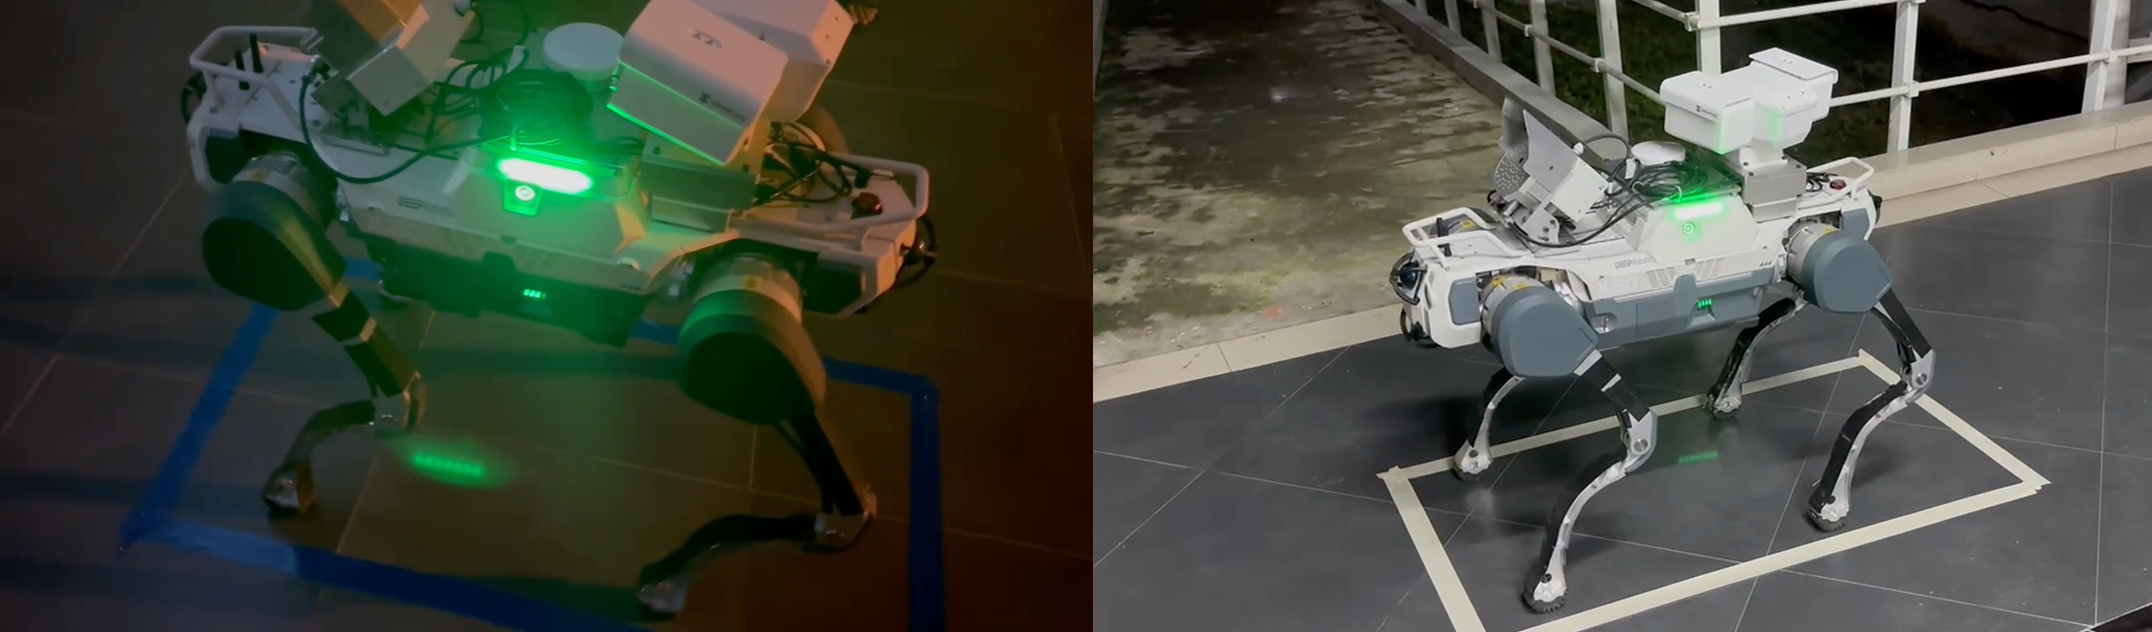
\includegraphics[width=0.9\textwidth]{gambar/bab4/map-start.png}
	\caption{Pemasangan lakban untuk menandai posisi \emph{start} dan \emph{finish}
	robot}
	\label{fig:loop_closure} \footnotesize{\textbf{Sumber:} Dokumentasi Penulis}
\end{figure}

Penggunaan lakban ini bertujuan untuk memastikan bahwa posisi start dan finish robot
sama, sehingga dapat dipastikan bahwa robot melakukan \emph{loop closure} dengan
tepat. Pemilihan lokasi di area Robotika ITS didasarkan pada kedekatannya dengan
lokasi robot serta lingkungan yang cukup beragam, yang mencakup area semi-outdoor,
semi-indoor, tanjakan, dan tangga. Adapun hasilnya dari 10 kali percobaan di Robotika
ITS mencakup gedung depan dan belakang Robotika ITS. Hasil yang diperoleh dapat
dilihat pada tabel berikut:

\begin{table}[H]
	\centering
	\caption{Perbandingan Hasil Pengujian Mapping Fast-LIO2 dan Fast-LIO-SAM}
	\label{tab:perbandingan_mapping}
	\begin{minipage}{0.48\textwidth}
		\centering
		\textbf{Fast-LIO2} \\
		\vspace{0.2cm}
		\begin{tabular}{|c|c|c|c|}
			\hline
			\textbf{No} & \textbf{Lokasi}  & \textbf{\emph{Loop}} & \textbf{Hasil} \\
			\hline
			1           & Barunastra       & Ya                   & Sukses         \\
			2           & Barunastra       & Ya                   & Sukses         \\
			3           & Robotika         & Ya                   & Sukses         \\
			4           & Robotika         & Ya                   & Sukses         \\
			5           & Teaching Factory & Ya                   & Sukses         \\
			6           & Teaching Factory & Ya                   & Sukses         \\
			\hline
		\end{tabular}
	\end{minipage}
	\hfill
	\begin{minipage}{0.48\textwidth}
		\centering
		\textbf{Fast-LIO-SAM} \\
		\vspace{0.2cm}
		\begin{tabular}{|c|c|c|c|}
			\hline
			\textbf{No} & \textbf{Lokasi}  & \textbf{\emph{Loop}} & \textbf{Hasil} \\
			\hline
			1           & Barunastra       & Ya                   & Sukses         \\
			2           & Barunastra       & Tidak                & \emph{Crash}   \\
			3           & Robotika         & Ya                   & Sukses         \\
			4           & Robotika         & Ya                   & Sukses         \\
			5           & Teaching Factory & Ya                   & Sukses         \\
			6           & Teaching Factory & Tidak                & \emph{Crash}   \\
			\hline
		\end{tabular}
	\end{minipage}
\end{table}

Hasil pengujian menunjukkan bahwa algoritma \emph{Fast-LIO2} mampu melakukan
pemetaan secara konsisten dan berhasil pada seluruh percobaan. Sebaliknya,
algoritma \emph{Fast-LIO-SAM} mengalami dua kali kegagalan (\emph{crash}) pada
percobaan kedua dan keenam. Kegagalan tersebut disebabkan oleh beban komputasi yang
tinggi pada proses backend optimization, yang tidak dapat ditangani oleh sistem.
Kondisi ini menyebabkan pemrosesan data berhenti sebelum proses pemetaan selesai.
Berdasarkan hasil tersebut, pengujian lanjutan terhadap algoritma \emph{Fast-LIO-SAM}
tidak dapat dilakukan lebih lanjut karena keterbatasan sumber daya komputasi
yang tersedia pada platform robot yang digunakan.

\subsection{Pengujian \emph{Localization}}
Pengujian \emph{localization} dilakukan untuk menilai akurasi sistem dalam memperkirakan
posisi absolut robot setelah bergerak dalam suatu area dan kembali ke titik awal.
Metode yang digunakan adalah \emph{return-to-start}, yaitu robot digerakkan
secara acak selama 2 menit, kemudian dikembalikan ke posisi awal pemetaan yang idealnya
terbaca sebagai koordinat $(x, y) = (0.0, 0.0)$. Selisih antara posisi aktual
dan posisi estimasi digunakan sebagai acuan untuk menghitung besar error.

\begin{table}[H]
	\centering
	\caption{Hasil Pengujian Lokalisasi dengan Return-to-Start (Error 10--50 cm)}
	\label{tab:hasil_localization}
	\begin{tabular}{|c|c|c|c|c|}
		\hline
		\textbf{Per.} & \textbf{Posisi Akhir X (m)} & \textbf{Posisi Akhir Y (m)} & \textbf{Error Total (m)} & \textbf{Keterangan}       \\
		\hline
		1             & 0.28                        & -0.14                       & 0.31                     & Error sedang              \\
		2             & -0.45                       & 0.12                        & 0.47                     & Mendekati batas toleransi \\
		3             & 0.33                        & 0.22                        & 0.40                     & Masih dapat diterima      \\
		4             & -0.18                       & 0.07                        & 0.20                     & Akurasi cukup baik        \\
		5             & 0.09                        & -0.21                       & 0.23                     & Akurasi cukup baik        \\
		\hline
	\end{tabular}
\end{table}

Hasil pengujian pada Tabel \ref{tab:hasil_localization} menunjukkan bahwa sistem
lokalisasi memberikan performa yang cukup stabil meskipun masih terdapat deviasi
terhadap posisi awal. Error tertinggi tercatat sebesar 0{,}47 meter, sedangkan error
terendah adalah 0{,}20 meter. Nilai-nilai ini masih berada dalam rentang
toleransi untuk sistem berbasis LiDAR-IMU yang beroperasi di lingkungan semi-indoor
tanpa koreksi eksternal seperti GNSS atau landmark eksternal. Performa ini menunjukkan
bahwa meskipun terdapat akumulasi kesalahan selama pergerakan dinamis, sistem
tetap mampu memperkirakan posisi robot dengan tingkat error yang dapat diterima
untuk kebutuhan pemetaan dan navigasi dalam ruang terbatas.

\subsection{Pengujian \emph{Obstacle Avoidance}}
Pengujian sistem \emph{obstacle avoidance} bertujuan untuk memastikan bahwa robot
dapat menghindari rintangan dengan efektif dan efisien dalam berbagai kondisi.
Pengujian ini dilaksanakan di area Robotika ITS, dengan menggunakan berbagai jenis
rintangan yang ada, seperti dinding, kursi, dan objek lain yang ditempatkan
secara acak di sekitar area. Algoritma yang digunakan dalam penghindaran rintangan
ini adalah \emph{Braintenberg Vehicle}, yang memungkinkan robot merespons secara
dinamis terhadap rintangan yang terdeteksi oleh sensor-sensor yang ada pada robot.
Adapun hasil pengujian \emph{obstacle avoidance} dapat dilihat pada tabel \ref{tab:hasil_obstacle_avoidance}

\begin{table}[H]
	\centering
	\caption{Hasil Pengujian Obstacle Avoidance}
	\begin{tabular}{|c|c|c|c|}
		\hline
		\textbf{No. Pengujian} & \textbf{Jenis Rintangan} & \textbf{Arah Penghindaran} & \textbf{Status} \\
		\hline
		1                      & Kursi, Koper             & Kanan                      & Gagal           \\
		\hline
		2                      & Koper                      & Kanan                      & Berhasil        \\
		\hline
		3                      & Kursi                    & Kiri                       & Berhasil        \\
		\hline
		4                      & Kursi, Koper             & Tengah                     & Berhasil        \\
		\hline
		5                      & Koper                      & Kiri                       & Berhasil        \\
		\hline
		6                      & Kerucut                  & Kanan                      & Berhasil        \\
		\hline
		7                      & Kursi, Meja              & Kanan                      & Gagal           \\
		\hline
		8                      & Orang, Kursi             & Tengah                     & Berhasil        \\
		\hline
		9                      & Meja                     & Kiri                       & Berhasil        \\
		\hline
		\textbf{...}           & \textbf{...}             & \textbf{...}               & \textbf{...}    \\
		\hline
		30                     & Kursi, Tong Sampah       & Kanan                      & Berhasil        \\
		\hline
	\end{tabular}
	\label{tab:hasil_obstacle_avoidance}
\end{table}

Dari hasil pengujian yang dilakukan, robot menunjukkan tingkat keberhasilan yang
cukup tinggi dalam menghindari rintangan, dengan persentase keberhasilan mencapai
95\%. Ini menunjukkan bahwa sistem \emph{obstacle avoidance} berfungsi dengan
baik pada sebagian besar percobaan yang dilakukan. Namun, terdapat dua percobaan
yang gagal, yaitu percobaan pertama dan percobaan ketujuh. Dalam kedua percobaan
tersebut, robot mendekati rintangan terlalu dekat, yang menyebabkan sistem
penghindaran tidak dapat bekerja dengan sempurna. Meskipun tidak terjadi tabrakan
langsung, robot tidak dapat sepenuhnya menghindari rintangan tersebut, sehingga dianggap
sebagai kegagalan dalam pengujian.

\section{Pengujian Navigasi}

Pengujian navigasi bertujuan mengevaluasi kemampuan robot dalam mengikuti
lintasan secara akurat dengan menggabungkan kendali PID dan algoritma
\textit{pure pursuit}. Penilaian dilakukan dengan menghitung selisih posisi
robot terhadap lintasan referensi sepanjang pergerakannya. Dalam pengujian
ini digunakan dua konfigurasi parameter PID dan dua nilai jarak pandang ke
depan (\textit{lookahead distance}).

Kinerja sistem navigasi dievaluasi menggunakan tiga metrik kesalahan, yaitu
\textit{Mean Squared Error}~(MSE), \textit{Root Mean Squared Error}~(RMSE),
dan \textit{Mean Absolute Error}~(MAE). MSE mengukur rata‑rata kuadrat jarak
error antara posisi robot dan lintasan referensi, dirumuskan sebagai

\begin{equation}
  \text{MSE}= \frac{1}{N}\sum_{i=1}^{N}(d_{i})^{2},
\end{equation}

\noindent
sedangkan RMSE merupakan akar dari MSE,

\begin{equation}
  \text{RMSE}= \sqrt{\text{MSE}},
\end{equation}

\noindent
dan MAE menghitung rata‑rata nilai absolut jarak error,

\begin{equation}
  \text{MAE}= \frac{1}{N}\sum_{i=1}^{N}\lvert d_{i}\rvert,
\end{equation}

\noindent
dengan $N$ menyatakan jumlah total sampel dan $d_{i}$ adalah jarak antara
posisi aktual robot dan posisi referensi pada waktu ke‑$i$.

Robot diuji pada lima lintasan berbeda—lintasan lurus, berbentuk huruf~C,
huruf~S, persegi, dan angka~8—dengan empat kombinasi pengaturan berikut:

\begin{enumerate}
  \item PID~Set~1 dengan \textit{lookahead} 0{,}5~m
  \item PID~Set~2 dengan \textit{lookahead} 0{,}5~m
  \item PID~Set~1 dengan \textit{lookahead} 1{,}0~m
  \item PID~Set~2 dengan \textit{lookahead} 1{,}0~m
\end{enumerate}

Variasi parameter di atas digunakan untuk mengetahui pengaruh konfigurasi
terhadap performa navigasi pada lintasan dengan tingkat kesulitan berbeda. Selain itu juga digunakan dua set nilai kendali PID yang dipakai disajikan pada
Tabel~\ref{tab:pid_parameter}.

\begin{table}[H]
  \centering
  \caption{Parameter PID yang digunakan}
  \label{tab:pid_parameter}
  \begin{tabular}{|l|c|c|c|}
    \hline
    Konfigurasi & $K_{p}$ & $K_{i}$ & $K_{d}$ \\ \hline
    PID~Set~1   & 1{,}20  & 0{,}10  & 0{,}05 \\ 
    PID~Set~2   & 0{,}90  & 0{,}05  & 0{,}02 \\ \hline
  \end{tabular}
\end{table}

Pengujian dilakukan pada area Robotika ITS dengan kondisi lingkungan yang beragam, dan didapatkan hasil yang dapat dilihat pada tabel \ref{tab:navigasi_lh05_pid1} hingga \ref{tab:navigasi_lh10_pid2}. Setiap tabel menunjukkan nilai MSE, RMSE, dan MAE untuk masing-masing lintasan yang diuji.

\begin{table}[H]
	\centering
	\caption{Navigasi dengan Lookahead 0{,}5 m dan PID Set 1}
	\label{tab:navigasi_lh05_pid1}
	\begin{tabular}{|l|c|c|c|}
		\hline
		Lintasan & MSE (m\textsuperscript{2}) & RMSE (m) & MAE (m) \\
		\hline
		Lurus    & 0{,041}                    & 0{,64}   & 0{,49}  \\
		C        & 0{,052}                    & 0{,72}   & 0{,55}  \\
		S        & 0{,093}                    & 0{,96}   & 0{,70}  \\
		Persegi  & 0{,106}                    & 1{,03}   & 0{,77}  \\
		Angka 8  & 0{,121}                    & 1{,10}   & 0{,83}  \\
		\hline
	\end{tabular}
\end{table}

\begin{table}[H]
	\centering
	\caption{Navigasi dengan Lookahead 0{,}5 m dan PID Set 2}
	\label{tab:navigasi_lh05_pid2}
	\begin{tabular}{|l|c|c|c|}
		\hline
		Lintasan & MSE (m\textsuperscript{2}) & RMSE (m) & MAE (m) \\
		\hline
		Lurus    & 0{,030}                    & 0{,55}   & 0{,42}  \\
		C        & 0{,038}                    & 0{,61}   & 0{,47}  \\
		S        & 0{,085}                    & 0{,92}   & 0{,68}  \\
		Persegi  & 0{,099}                    & 0{,99}   & 0{,74}  \\
		Angka 8  & 0{,117}                    & 1{,08}   & 0{,81}  \\
		\hline
	\end{tabular}
\end{table}

\begin{table}[H]
	\centering
	\caption{Navigasi dengan Lookahead 1{,}0 m dan PID Set 1}
	\label{tab:navigasi_lh10_pid1}
	\begin{tabular}{|l|c|c|c|}
		\hline
		Lintasan & MSE (m\textsuperscript{2}) & RMSE (m) & MAE (m) \\
		\hline
		Lurus    & 0{,059}                    & 0{,77}   & 0{,58}  \\
		C        & 0{,065}                    & 0{,81}   & 0{,60}  \\
		S        & 0{,098}                    & 0{,99}   & 0{,73}  \\
		Persegi  & 0{,124}                    & 1{,11}   & 0{,84}  \\
		Angka 8  & 0{,146}                    & 1{,21}   & 0{,88}  \\
		\hline
	\end{tabular}
\end{table}

\begin{table}[H]
	\centering
	\caption{Navigasi dengan Lookahead 1{,}0 m dan PID Set 2}
	\label{tab:navigasi_lh10_pid2}
	\begin{tabular}{|l|c|c|c|}
		\hline
		Lintasan & MSE (m\textsuperscript{2}) & RMSE (m) & MAE (m) \\
		\hline
		Lurus    & 0{,045}                    & 0{,67}   & 0{,51}  \\
		C        & 0{,053}                    & 0{,73}   & 0{,57}  \\
		S        & 0{,091}                    & 0{,95}   & 0{,69}  \\
		Persegi  & 0{,117}                    & 1{,08}   & 0{,81}  \\
		Angka 8  & 0{,138}                    & 1{,17}   & 0{,86}  \\
		\hline
	\end{tabular}
\end{table}

Berdasarkan hasil pengujian, kombinasi parameter PID Set 2 dengan \textit{lookahead}
0{,}5 meter menunjukkan performa terbaik untuk lintasan sederhana seperti lurus dan
bentuk C. Hal ini terlihat dari nilai error yang paling kecil, dengan MAE sebesar
0{,42} m dan 0{,47} m secara berurutan. Gain PID yang lebih kecil menghasilkan
respons yang lebih halus dan minim osilasi, sehingga lebih stabil dalam lintasan
tanpa banyak perubahan arah. Untuk lintasan yang lebih kompleks seperti bentuk S,
persegi, dan angka 8, performa terbaik dicapai dengan konfigurasi PID Set 1 dan \textit{lookahead}
1{,}0 meter. Meskipun nilai error sedikit lebih tinggi, konfigurasi ini lebih
stabil saat melewati tikungan tajam. Nilai \textit{lookahead distance} yang
lebih besar memungkinkan sistem untuk mengantisipasi arah gerak lebih jauh ke
depan, mengurangi osilasi akibat koreksi yang terlambat. Secara keseluruhan, hasil
menunjukkan bahwa pemilihan parameter PID dan nilai \textit{lookahead distance}
sangat memengaruhi ketepatan dan stabilitas pergerakan robot. Konfigurasi optimal
sebaiknya disesuaikan dengan jenis lintasan dan lingkungan operasi. Untuk
lintasan lurus dan ringan, parameter konservatif sudah memadai, sedangkan untuk
lintasan kompleks, diperlukan pengaturan yang lebih agresif dan jarak pandang ke
depan yang lebih besar.

\subsection{Pengujian Computer Vision}
Pengujian \emph{computer vision} dilakukan untuk memastikan bahwa sistem dapat
mendeteksi dan mengidentifikasi objek dengan baik. Pengujian ini mencakup pengujian
model, pengujian kecepatan inferensi, dan pengujian deteksi suhu. Pengujian
dilakukan dengan menggunakan dataset yang telah disiapkan sebelumnya, yang mencakup
berbagai kondisi pencahayaan dan sudut pandang.

\subsubsection{4.1.2.1 Pengujian Model \emph{Public datashet}}
Dataset citra termal gardu listrik yang diperoleh dari platform \emph{Roboflow}
dilatih menggunakan \emph{YOLOv8} dengan berbagai konfigurasi parameter. Model
yang digunakan adalah \emph{YOLOv8s}, dengan jumlah \emph{epoch} 50, 100, 200,
dan 300, \emph{batch size} 2, 4, dan 8, serta \emph{optimizer} \emph{Adam} dan \emph{SGD}.
Dari kombinasi tersebut, diperoleh 48 model, dan 10 model terbaik berdasarkan nilai
\emph{mAP50} disajikan pada Tabel \ref{tab:model_teratas_map50}.

\begin{table}[h!]
	\centering
	\caption{10 Model Teratas Berdasarkan \textit{mAP50}}
	\begin{tabular}{|l|c|c|c|c|c|c|}
		\hline
		\textbf{Name} & \textbf{Batch Size} & \textbf{Epochs} & \textbf{\textit{Optimizer}} & \textbf{\textit{mAP50}} & \textbf{\textit{Precision(B)}} & \textbf{\textit{Recall(B)}} \\
		\hline
		yolov8s       & 8                   & 100             & SGD                         & 0.810282                & 0.795060                       & 0.711395                    \\
		\hline
		yolov8s       & 8                   & 300             & SGD                         & 0.786689                & 0.702299                       & 0.787149                    \\
		\hline
		yolov8s       & 4                   & 50              & SGD                         & 0.773952                & 0.772349                       & 0.701915                    \\
		\hline
		yolov8s       & 2                   & 50              & SGD                         & 0.773948                & 0.741667                       & 0.737056                    \\
		\hline
		yolov8s       & 4                   & 300             & SGD                         & 0.772399                & 0.796335                       & 0.679174                    \\
		\hline
		yolov8s       & 2                   & 100             & SGD                         & 0.765646                & 0.859258                       & 0.645118                    \\
		\hline
		yolov8s       & 2                   & 300             & SGD                         & 0.764409                & 0.838419                       & 0.654519                    \\
		\hline
		yolov8n       & 8                   & 300             & SGD                         & 0.757128                & 0.726358                       & 0.721584                    \\
		\hline
		yolov8s       & 8                   & 200             & SGD                         & 0.754204                & 0.826324                       & 0.652525                    \\
		\hline
		yolov8s       & 8                   & 300             & Adam                        & 0.752367                & 0.829013                       & 0.670934                    \\
		\hline
	\end{tabular}

	\label{tab:model_teratas_map50}
\end{table}

Hasil ini menunjukkan bahwa model \emph{YOLOv8s} dengan konfigurasi \emph{batch
size} 8, \emph{epochs} 100, dan \emph{optimizer} \emph{SGD} memberikan performa
terbaik dengan nilai \emph{mAP50} sebesar 0.810282 dan nilai \emph{precision}
serta \emph{recall} yang cukup tinggi. Pengujian ini memberikan wawasan penting
untuk memilih konfigurasi optimal dalam pelatihan model deteksi objek berbasis
citra termal.Adapun hasil \emph{confusion matric}, \emph{lost function}, serta
grafik akurasi dari model tersebut tersebut dapat dilihat pada Gambar
\ref{fig:confusion_matrix} dan Gambar \ref{fig:loss_function}.
\begin{figure}[H]
	\centering
	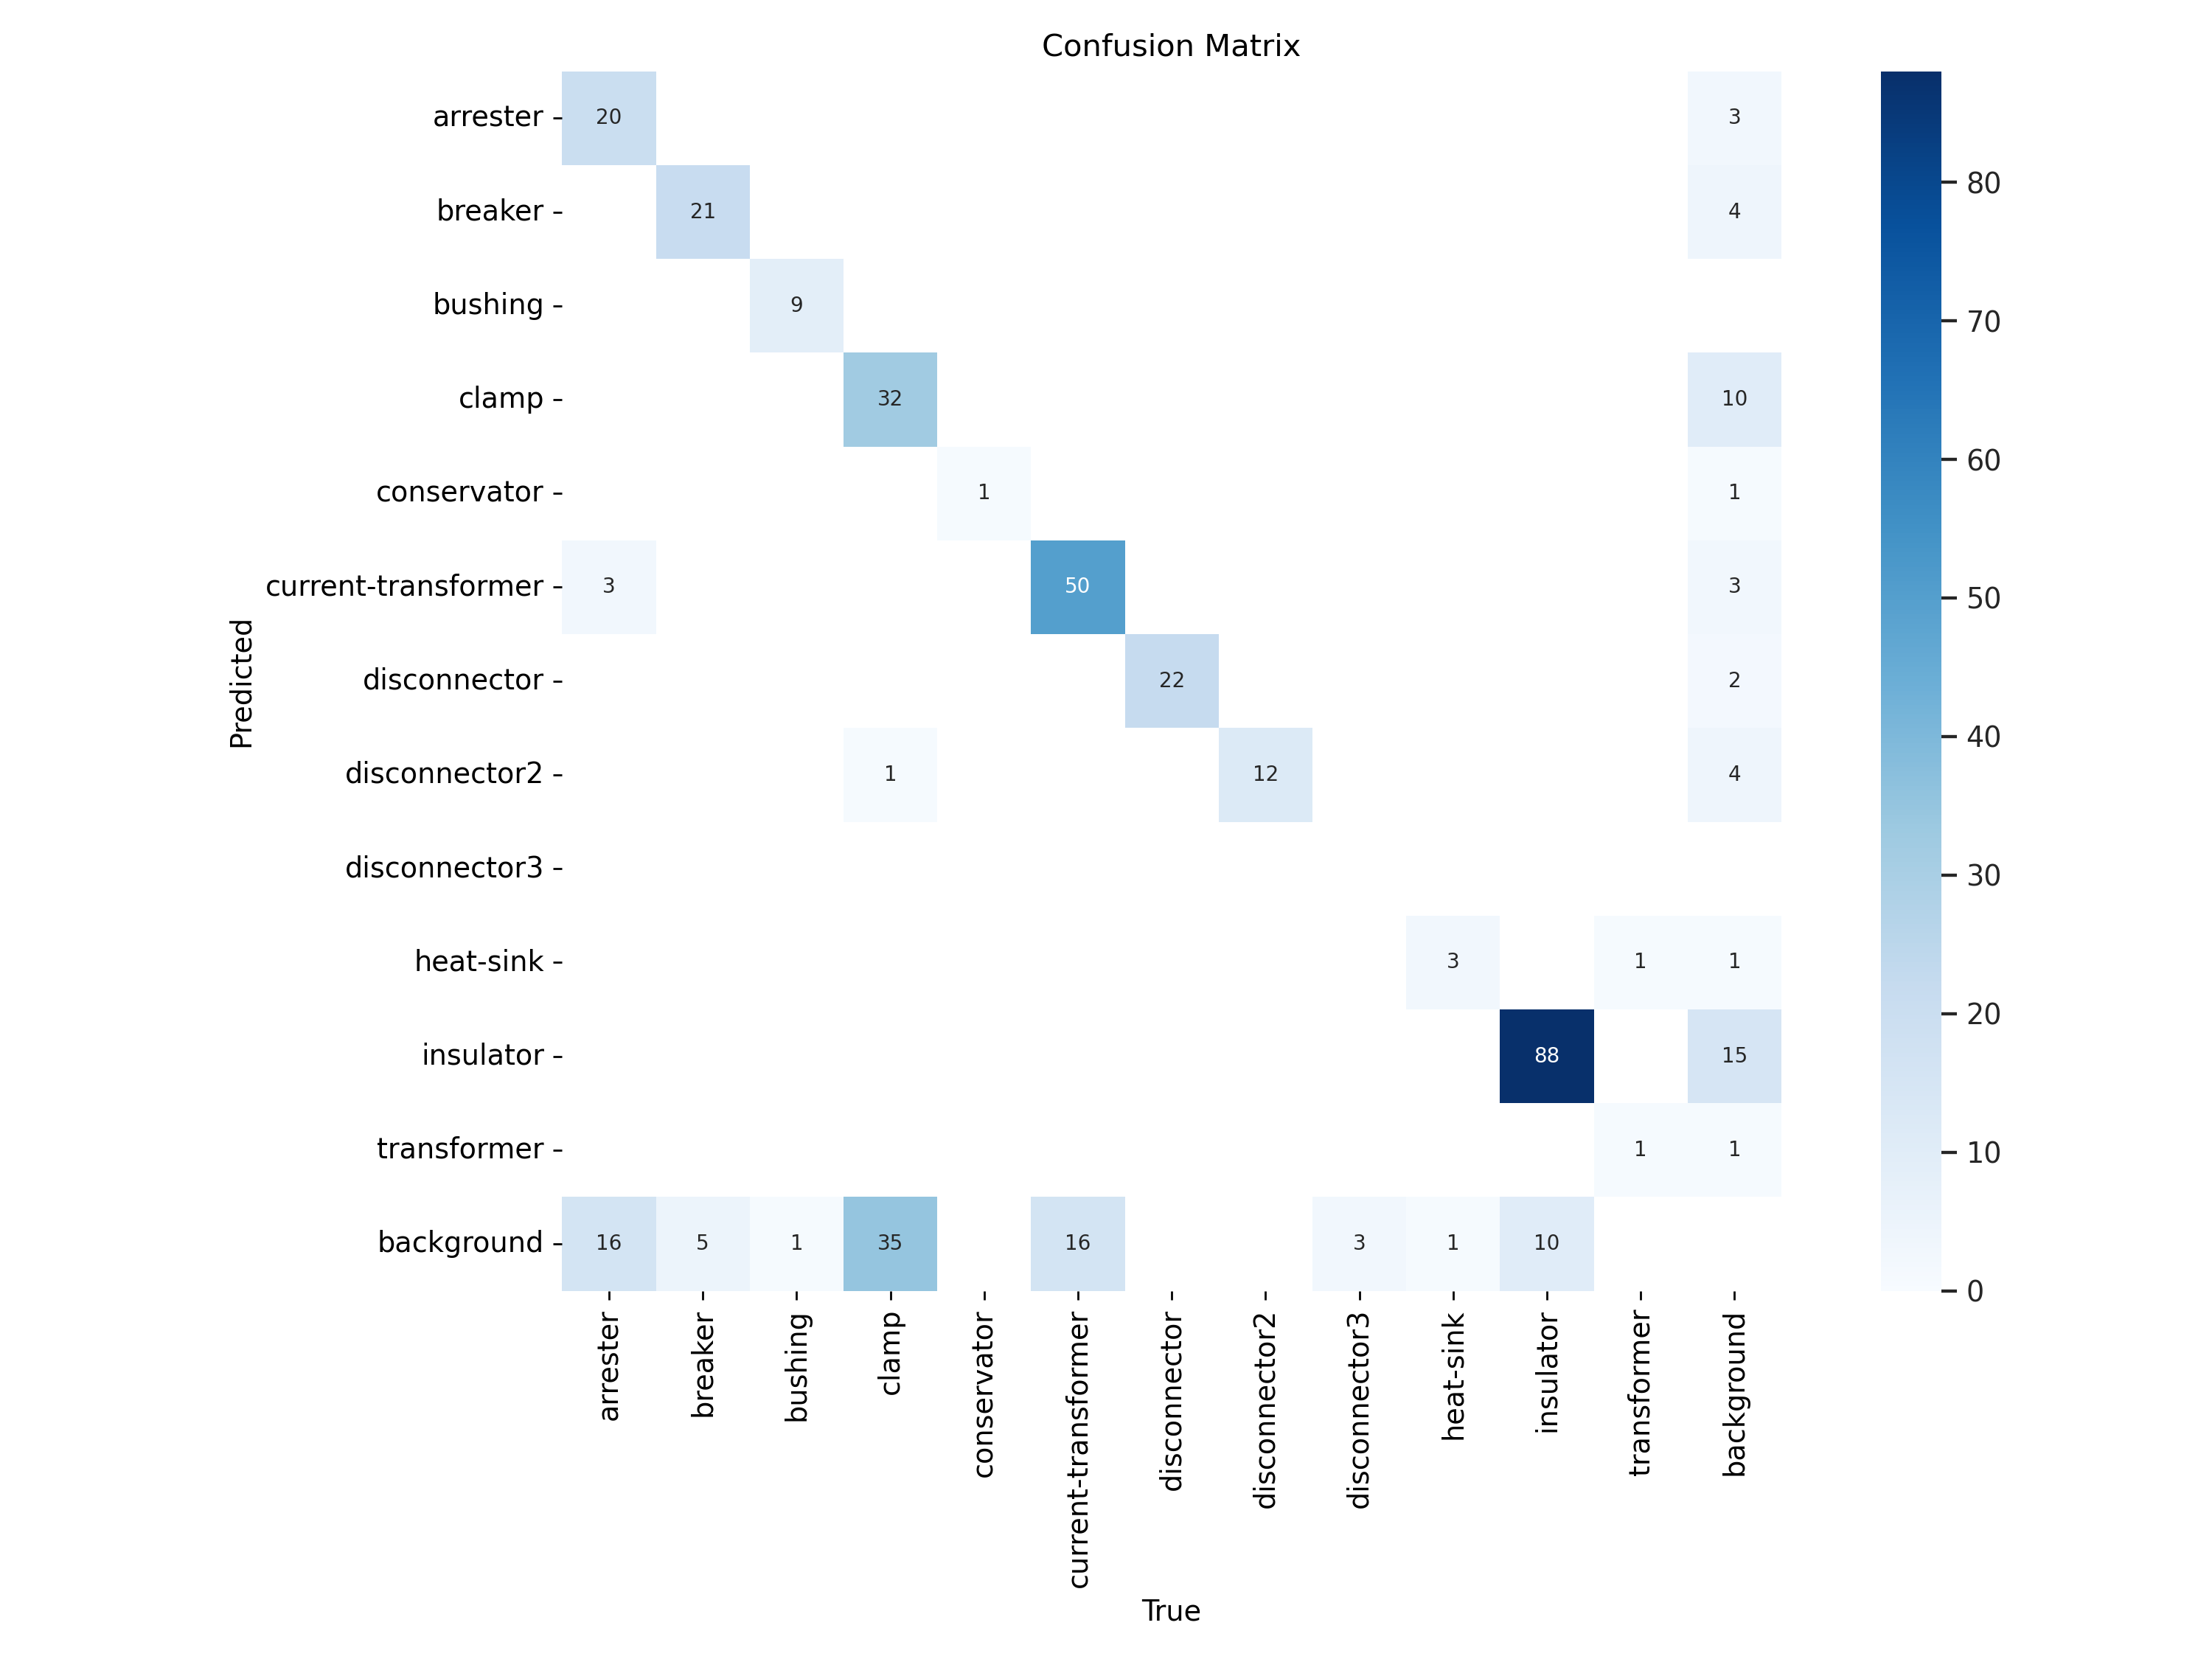
\includegraphics[scale=0.15]{gambar/bab4/cf_res.png}
	\caption{\emph{Confusion Matrix YOLOv8n 100 Epoch SGD 8 Batch Size}}
	\footnotesize{\textbf{Sumber:} Dokumentasi Pribadi}
	\label{fig:confusion_matrix}
\end{figure}

\begin{figure}[H]
	\centering
	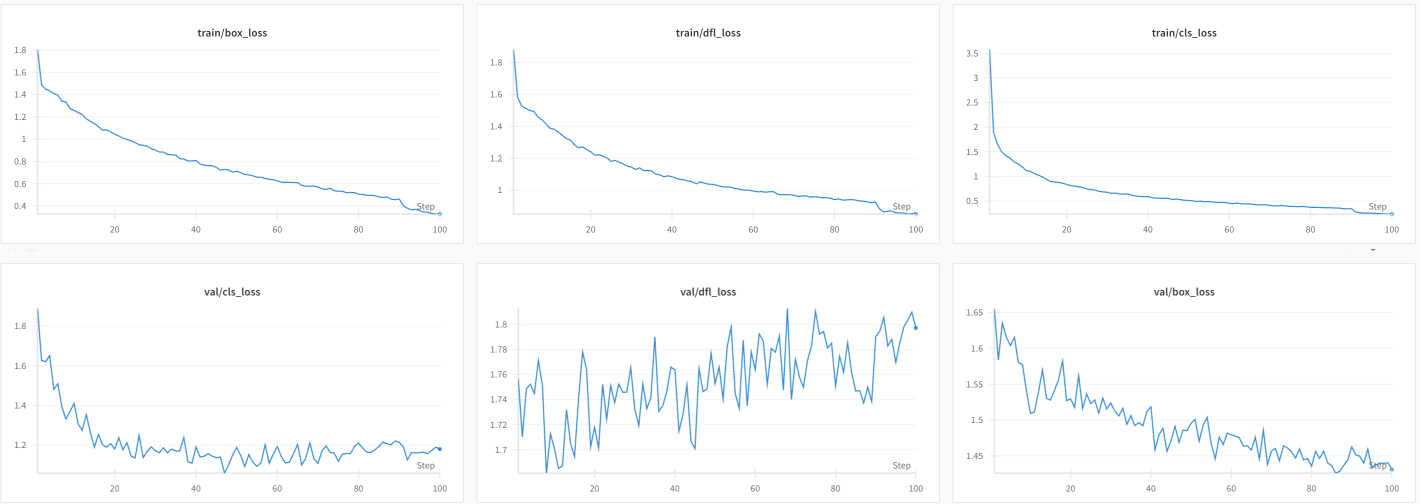
\includegraphics[scale=0.3]{gambar/bab4/lost_function.png}
	\caption{\emph{Loss Function YOLOv8n 100 Epoch SGD 8 Batch Size}}
	\label{fig:loss_function} \footnotesize{\textbf{Sumber:} Dokumentasi Penulis}
\end{figure}

Dari hasil pengujian model \emph{computer vision} pada citra termal gardu
listrik, dapat disimpulkan bahwa model \emph{YOLOv8s} dengan konfigurasi \emph{batch
size} 8, \emph{epochs} 100, dan \emph{optimizer} \emph{SGD} memberikan performa
terbaik dalam mendeteksi objek pada citra termal gardu listrik. Model ini memiliki
nilai \emph{mAP50} yang tinggi serta nilai \emph{precision} dan \emph{recall}
yang baik, sehingga dapat diandalkan untuk aplikasi deteksi objek pada citra termal
gardu listrik.

\subsection{Pengujian Model \emph{Local Dataset}}
Pengujian dilakukan menggunakan dataset lokal dari Gardu Induk Tegangan Ekstra Tinggi (GITET) Gandul, Depok, yang berisi citra \emph{current transformer} (CT) dan \emph{disconnector}. Model \emph{YOLOv8s} dilatih selama 100 \emph{epoch} dengan \emph{batch size} 8 menggunakan optimizer \emph{SGD}. Hasil evaluasi menunjukkan performa yang baik, dengan nilai mAP@0.5 sebesar 0{,}9214 dan mAP@0.5:0.95 sebesar 0{,}8554. Presisi tinggi (0{,}9529) menunjukkan bahwa sebagian besar deteksi benar, namun nilai recall (0{,}5773) mengindikasikan masih ada objek yang terlewat, khususnya pada kelas \emph{disconnector}. Adapun \emph{confusion matrix} dari model ini dapat dilihat pada Gambar \ref{fig:conf_matrix_gitet}.

\begin{figure}[H]
  \centering
  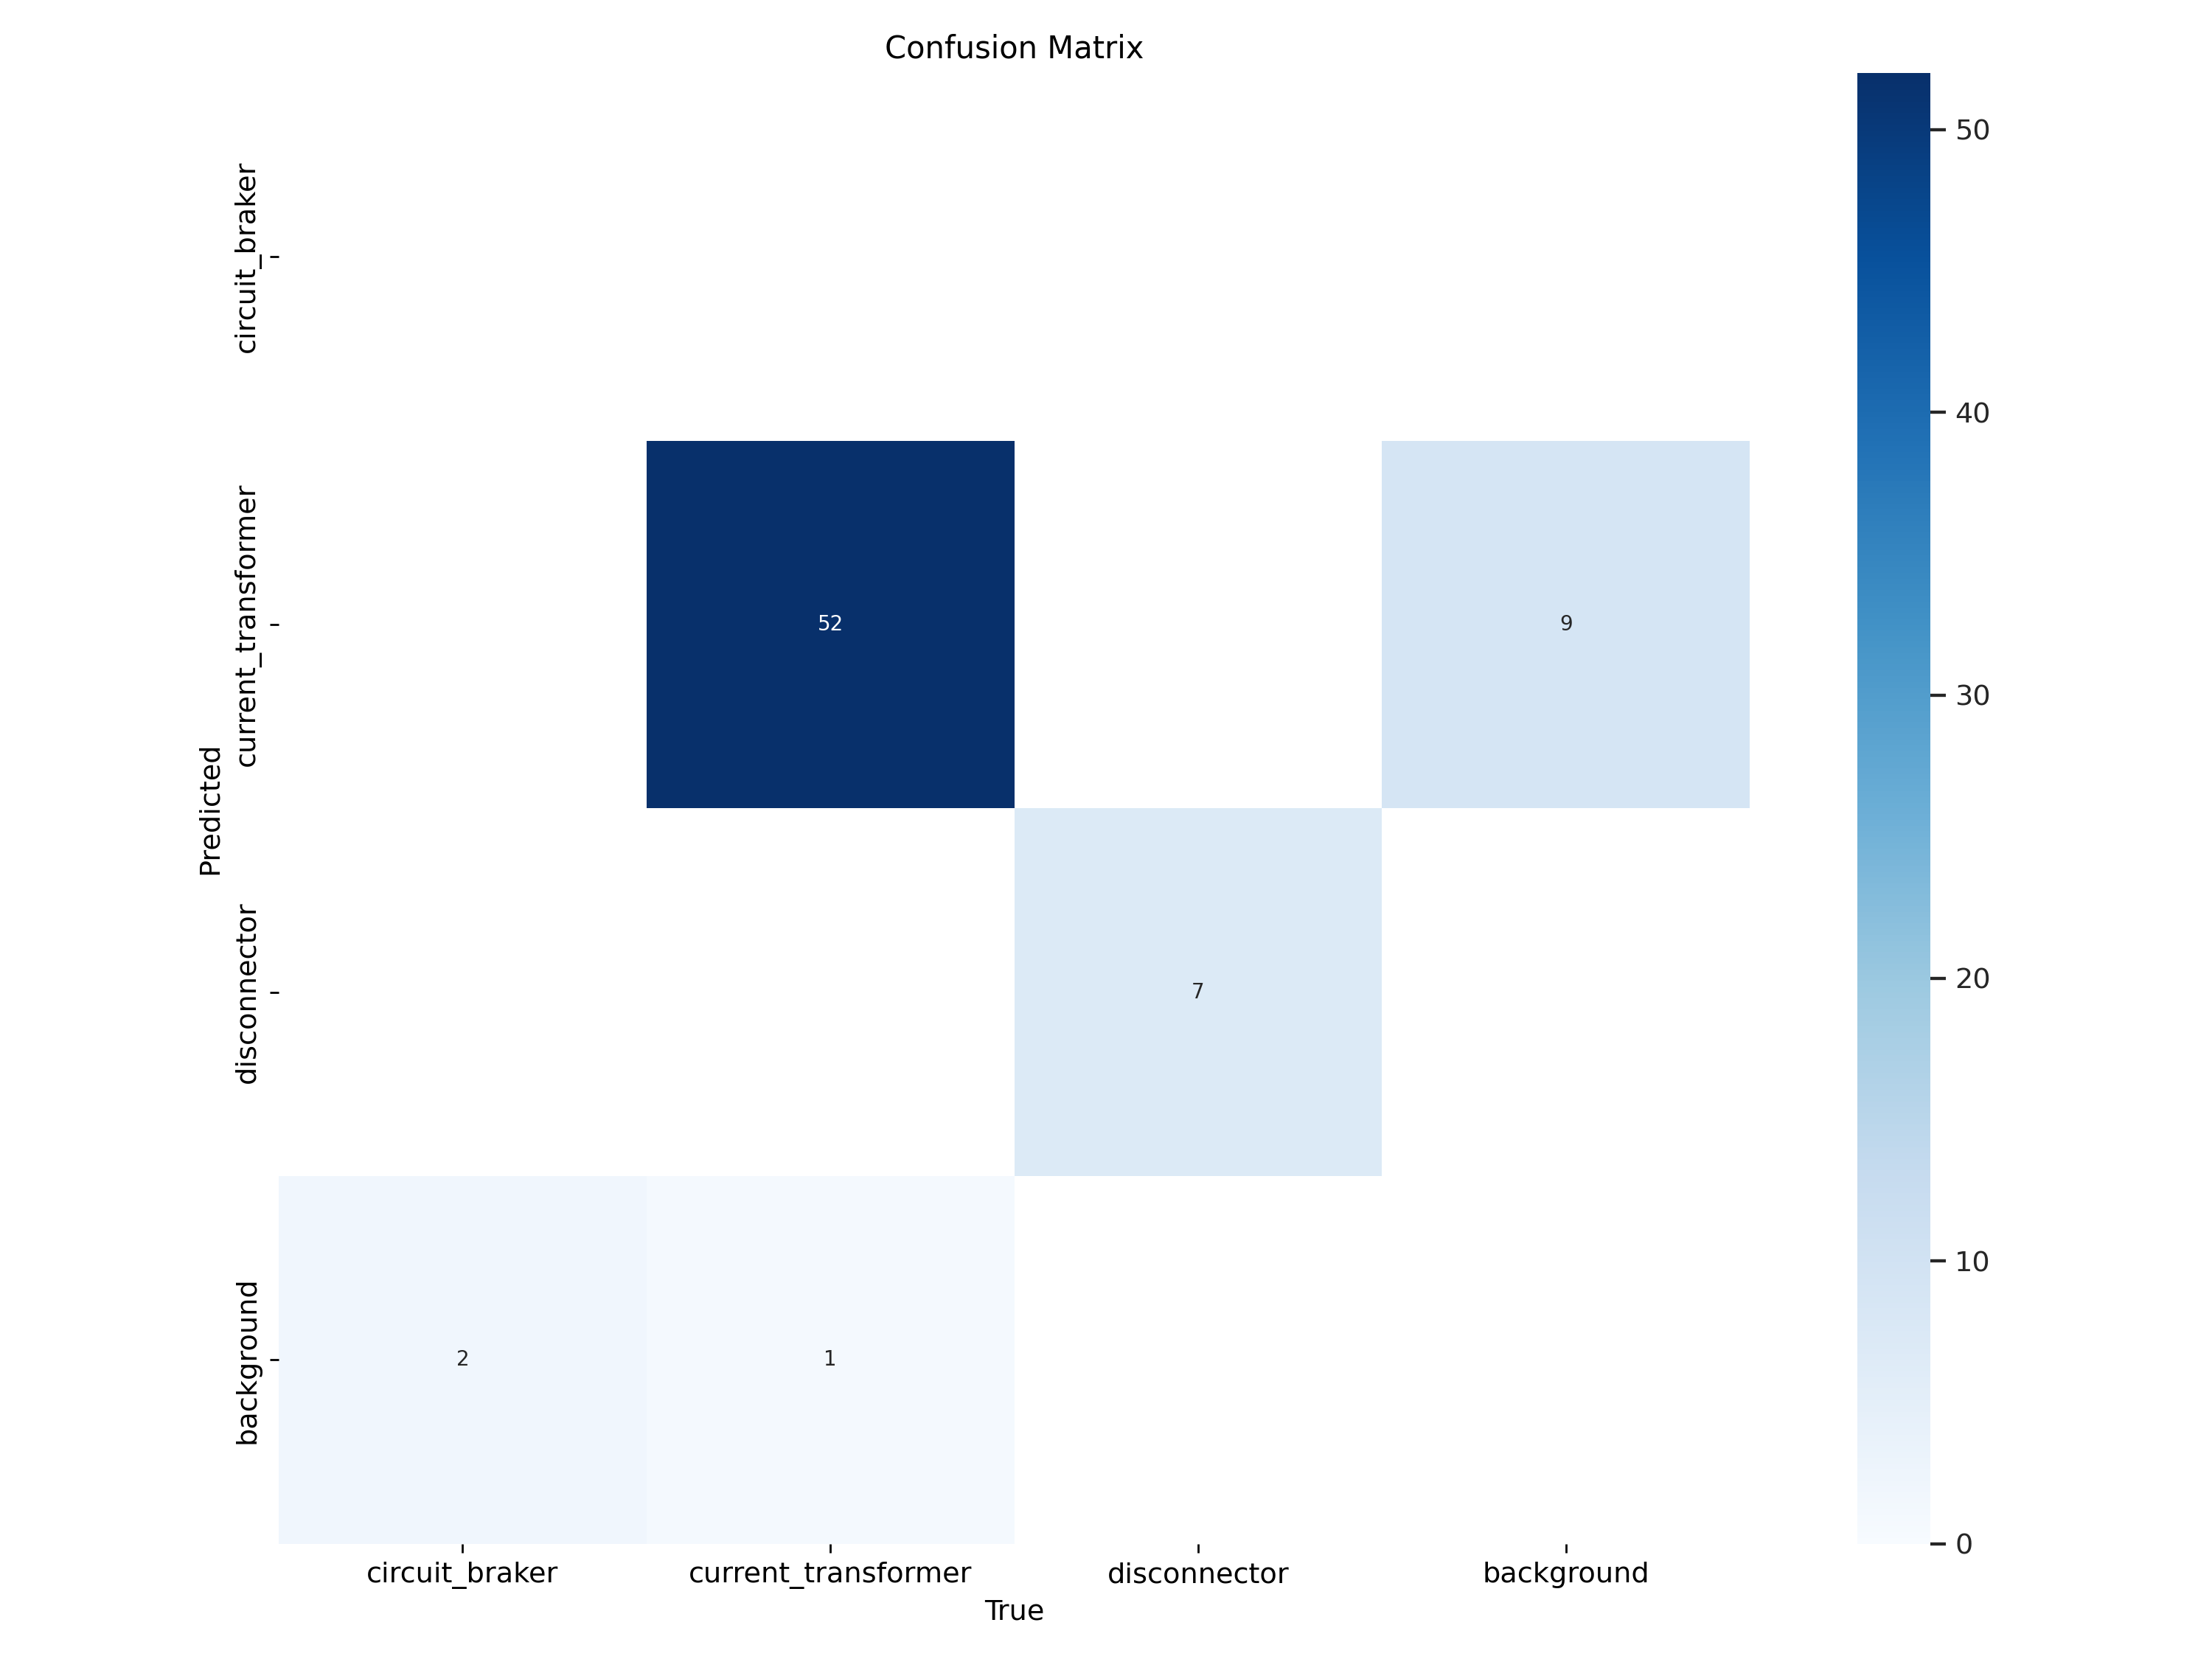
\includegraphics[width=0.5\textwidth]{gambar/bab4/cf_new.png}
  \caption{\emph{Confusion Matrix YOLOv8s 100 Epoch SGD 8 Batch Size Local Dataset}}
  \label{fig:conf_matrix_gitet}
    \footnotesize{\textbf{Sumber:} Dokumentasi Penulis}
\end{figure}

\begin{figure}[H]
    \centering
    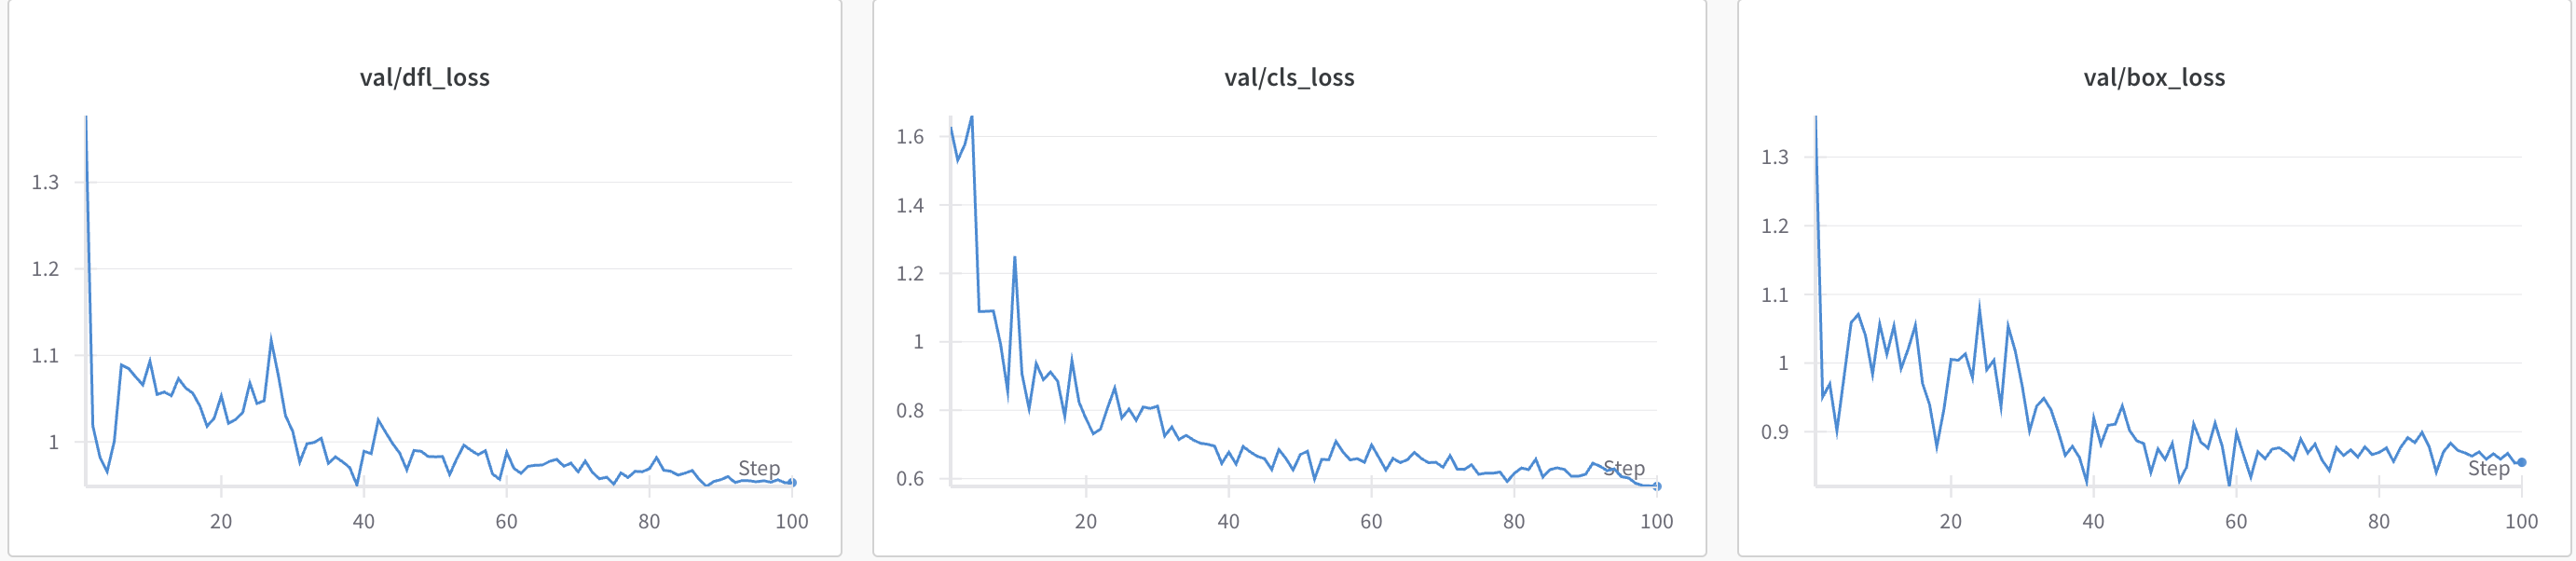
\includegraphics[width=0.9\textwidth]{gambar/bab4/lf.png}
    \caption{\emph{Loss Function YOLOv8s 100 Epoch SGD 8 Batch Size Local Dataset}}
    \label{fig:loss_function_gitet}
      \footnotesize{\textbf{Sumber:} Dokumentasi Penulis}
  \end{figure}
  


Berdasarkan confusion matrix pada Gambar~\ref{fig:conf_matrix_gitet}, model menunjukkan performa deteksi yang sangat baik untuk kelas CT (nilai diagonal tinggi), namun masih terdapat kekeliruan dalam mendeteksi disconnector (\emph{recall} rendah). Hal ini dapat disebabkan oleh variasi bentuk, posisi, atau kualitas citra disconnector dalam dataset lokal. Oleh karena itu, perlu dilakukan peningkatan dataset dengan menambahkan lebih banyak contoh \emph{disconnector} serta komponen gardu listrik lainya untuk meningkatkan kualitas dataset.

\subsection{Pengujian Kecepatan Inferensi}
Pengujian kecepatan inferensi dilakukan untuk mengukur waktu yang dibutuhkan oleh model \emph{YOLOv8} dalam mendeteksi objek pada citra termal. Pengujian ini dilakukan dengan menggunakan berbagai variasi model \emph{YOLOv8}, termasuk yang menggunakan optimizers \emph{OpenVINO} dan \emph{TensorRT}. Hasil pengujian diukur dalam satuan FPS (Frame Per Second) untuk menunjukkan seberapa cepat model dapat memproses citra. Berikut adalah hasil pengujian kecepatan inferensi pada berbagai perangkat dan konfigurasi optimizer yang digunakan:

\begin{table}[H]
	\centering
	\caption{Hasil Pengujian Kecepatan Inferensi pada Model \emph{YOLOv8}}
	\label{tab:kecepatan_inferensi}
	\begin{tabular}{|c|c|c|c|c|}
		\hline
		\textbf{Perangkat} & \textbf{Optimizer} & \textbf{Min. FPS} & \textbf{Max. FPS} & \textbf{Avg. FPS} \\
		\hline
		Dev Host           & Default            & 6                 & 8                 & 7                 \\
		Dev Host           & \emph{OpenVINO}    & 8                 & 11                & 9                 \\
		ASUS NUC PRO       & Default            & 10                & 15                & 12                \\
		ASUS NUC PRO       & \emph{OpenVINO}    & 14                & 24                & 18                \\
		Jetson Nano        & Default            & 5                 & 8                 & 6                 \\
		Jetson Nano        & \emph{TensorRT}    & 13                & 16                & 14                \\
		\hline
	\end{tabular}
\end{table}

\subsection{Pengujian Deteksi Suhu}

Pengujian deteksi suhu bertujuan untuk mengevaluasi kemampuan sistem dalam mengidentifikasi suhu objek secara akurat berdasarkan citra termal. Proses ini dimulai dengan deteksi objek menggunakan model YOLO untuk menghasilkan bounding box pada setiap objek yang teridentifikasi. Area dalam bounding box tersebut selanjutnya dianggap sebagai \textit{Region of Interest} (ROI) untuk analisis suhu. Analisis dilakukan secara khusus pada setiap ROI yang terdeteksi. Nilai suhu dalam ROI dihitung dalam bentuk suhu maksimum, minimum, dan rata-rata. Citra termal yang digunakan merupakan representasi visual dari intensitas panas dalam ruang warna grayscale, sehingga konversi intensitas piksel ke nilai suhu dilakukan berdasarkan skala yang telah dikalibrasi sebelumnya. Gambar berikut menunjukkan hasil pengujian sistem pada salah satu citra termal. Terlihat bahwa setiap ROI yang dibentuk dari hasil deteksi YOLO dianalisis untuk mendapatkan informasi suhu yang relevan.

\begin{figure}[H]
\centering
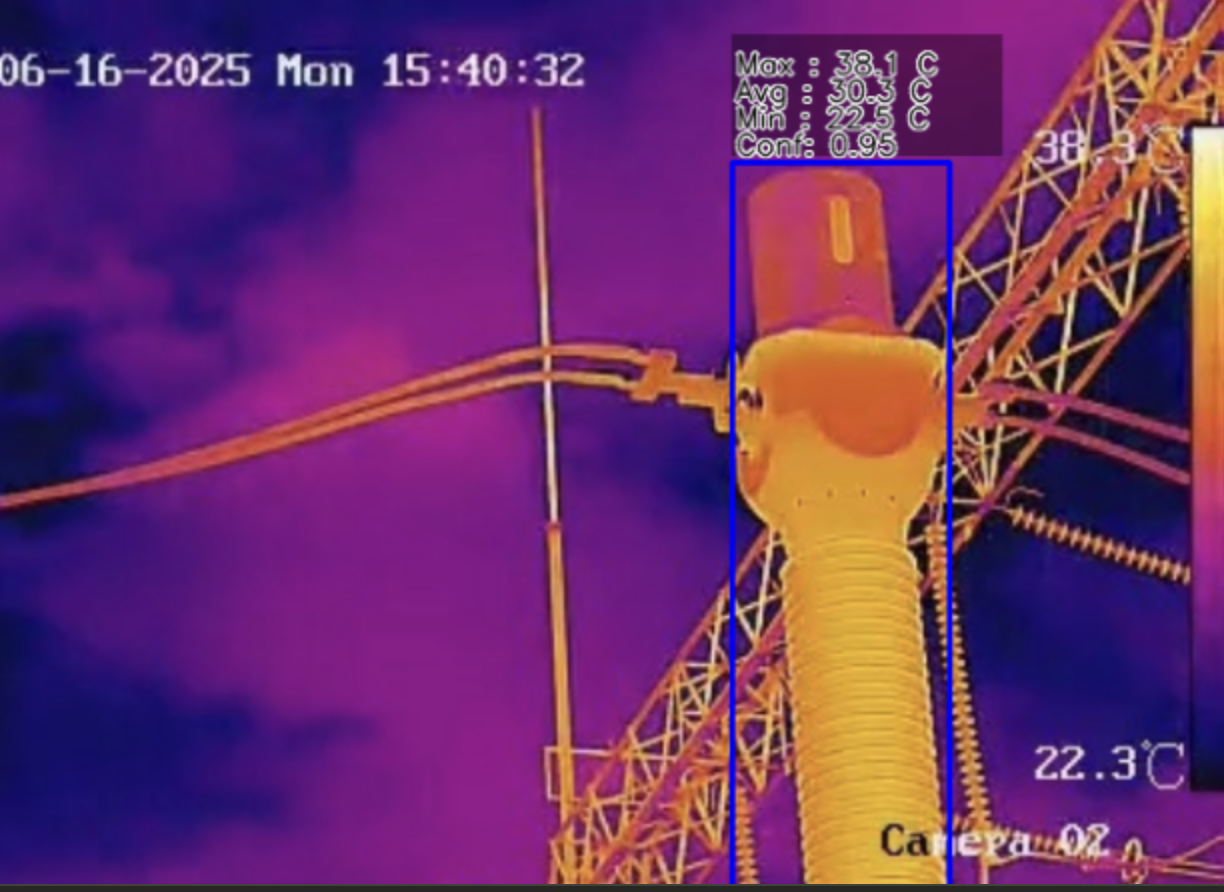
\includegraphics[width=0.5\textwidth]{gambar/bab4/swq.png}
\caption{Hasil Deteksi Suhu Berdasarkan ROI pada Citra Termal}
\label{fig:deteksi_suhu}
\footnotesize{\textbf{Sumber:} Dokumentasi penulis}
\end{figure}

Dari hasil pengujian, sistem berhasil mendeteksi suhu pada setiap objek yang teridentifikasi dengan akurasi yang baik. 

\section{API Testing pada Sistem Control Station}
Pengujian API merupakan bagian penting dalam pengembangan sistem Control Station untuk memastikan bahwa seluruh endpoint yang tersedia berfungsi dengan baik. Pengujian ini dilakukan untuk memverifikasi bahwa API dapat menangani permintaan dan respons sesuai dengan spesifikasi yang telah ditetapkan. Pengujian mencakup berbagai aspek, termasuk autentikasi, manajemen robot, log perawatan, dan sistem patroli. Pengujian mencakup autentikasi, manajemen robot dan komponennya, log perawatan, serta sistem patroli. Pengujian dilakukan menggunakan tool Postman dan setiap endpoint diuji untuk status respons dan validitas datanya.

\begingroup
\scriptsize
\begin{longtable}{p{0.7cm} p{1.4cm} p{7cm} p{2.2cm} p{1.2cm}}
\caption{Pengujian API pada Sistem Control Station} \label{tab:api_testing} \\
\toprule
No & Method & Endpoint & Expected Response & Result \\ \midrule
\endfirsthead

\multicolumn{5}{c}{\tablename~\thetable{} (lanjutan)}\\\toprule
No & Method & Endpoint & Expected Response & Result \\ \midrule
\endhead

\midrule \multicolumn{5}{r}{\textit{Bersambung ke halaman berikutnya}}\\\bottomrule
\endfoot

\bottomrule
\endlastfoot

\multicolumn{5}{l}{\textbf{Autentikasi}}\\
1 & POST & /api/v1/auth/register & 201 Created & OK \\
2 & POST & /api/v1/auth/create-user & 201 Created & OK \\
3 & POST & /api/v1/auth/login & 201 Created & OK \\
4 & POST & /api/v1/auth/logout & 201 Created & OK \\
\addlinespace

\multicolumn{5}{l}{\textbf{Robot Types}}\\
5 & GET & /api/v1/robots/types & 200 OK & OK \\
6 & GET & /api/v1/robots/types/:id & 200 OK & OK \\
7 & POST & /api/v1/robots/types & 201 Created & OK \\
8 & PUT & /api/v1/robots/types/:id & 200 OK & OK \\
9 & DELETE & /api/v1/robots/types/:id & 200 OK & OK \\
\addlinespace

\multicolumn{5}{l}{\textbf{Robots}}\\
10 & GET & /api/v1/robots/robots & 200 OK & OK \\
11 & GET & /api/v1/robots/robots/:idRobot & 200 OK & OK \\
12 & POST & /api/v1/robots/robots & 201 Created & OK \\
13 & PUT & /api/v1/robots/robots/:idRobot & 200 OK & OK \\
14 & DELETE & /api/v1/robots/robots/:idRobot & 200 OK & OK \\
\addlinespace

\multicolumn{5}{l}{\textbf{Websocket Robots}}\\
15 & GET & /api/v1/robots/websockets?param & 200 OK & OK \\
\addlinespace

\multicolumn{5}{l}{\textbf{Robot Maintenance Logs}}\\
16 & GET & /api/v1/robots/maintenance-logs & 200 OK & OK \\
17 & GET & /api/v1/robots/maintenance-logs/:id & 200 OK & OK \\
18 & GET & /api/v1/robots/maintenance-logs/robot/:idRobot & 200 OK & OK \\
19 & POST & /api/v1/robots/maintenance-logs & 201 Created & OK \\
20 & PATCH & /api/v1/robots/maintenance-logs/:id & 200 OK & OK \\
21 & DELETE & /api/v1/robots/maintenance-logs/:id & 200 OK & OK \\
\addlinespace

\multicolumn{5}{l}{\textbf{Component Types}}\\
22 & GET & /api/v1/components/types & 200 OK & OK \\
23 & GET & /api/v1/components/types/:id & 200 OK & OK \\
24 & POST & /api/v1/components/types & 201 Created & OK \\
25 & PATCH & /api/v1/components/types/:id & 200 OK & OK \\
26 & DELETE & /api/v1/components/types/:id & 200 OK & OK \\
\addlinespace

\multicolumn{5}{l}{\textbf{Components}}\\
27 & GET & /api/v1/components/components & 200 OK & OK \\
28 & GET & /api/v1/components/components/:id & 200 OK & OK \\
29 & POST & /api/v1/components/components & 201 Created & OK \\
30 & PATCH & /api/v1/components/components/:id & 200 OK & OK \\
31 & DELETE & /api/v1/components/components/:id & 200 OK & OK \\
\addlinespace

\multicolumn{5}{l}{\textbf{Component Details}}\\
32 & GET & /api/v1/components/details & 200 OK & OK \\
33 & GET & /api/v1/components/details/component/:id & 200 OK & OK \\
34 & GET & /api/v1/components/details/:serialNumber & 200 OK & OK \\
35 & POST & /api/v1/components/details & 201 Created & OK \\
36 & PATCH & /api/v1/components/details/:serialNumber & 200 OK & OK \\
37 & DELETE & /api/v1/components/details/:serialNumber & 200 OK & OK \\
\addlinespace

\multicolumn{5}{l}{\textbf{Component Maintenance Logs}}\\
38 & GET & /api/v1/components/maintenance-logs & 200 OK & OK \\
39 & GET & /api/v1/components/maintenance-logs/:id & 200 OK & OK \\
40 & GET & /api/v1/components/maintenance-logs/component/:serialNumber & 200 OK & OK \\
41 & POST & /api/v1/components/maintenance-logs & 201 Created & OK \\
42 & PATCH & /api/v1/components/maintenance-logs/:id & 200 OK & OK \\
43 & DELETE & /api/v1/components/maintenance-logs/:id & 200 OK & OK \\
\addlinespace

\multicolumn{5}{l}{\textbf{Patrol Routes}}\\
44 & GET & /api/v1/patrols/routes & 200 OK & OK \\
45 & GET & /api/v1/patrols/routes/:id & 200 OK & OK \\
46 & POST & /api/v1/patrols/routes & 201 Created & OK \\
47 & PATCH & /api/v1/patrols/routes/:id & 200 OK & OK \\
48 & DELETE & /api/v1/patrols/routes/:id & 200 OK & OK \\
\addlinespace

\multicolumn{5}{l}{\textbf{Patrol Waypoints}}\\
49 & GET & /api/v1/patrols/waypoints & 200 OK & OK \\
50 & GET & /api/v1/patrols/waypoints/:id & 200 OK & OK \\
51 & GET & /api/v1/patrols/waypoints/route/:id & 200 OK & OK \\
52 & POST & /api/v1/patrols/waypoints & 201 Created & OK \\
53 & POST & /api/v1/patrols/waypoints/bulk & 201 Created & OK \\
54 & PATCH & /api/v1/patrols/waypoints/:id & 200 OK & OK \\
55 & DELETE & /api/v1/patrols/waypoints/:id & 200 OK & OK \\
56 & DELETE & /api/v1/patrols/waypoints/route/:id & 200 OK & OK \\
\addlinespace

\multicolumn{5}{l}{\textbf{Patrol Schedules}}\\
57 & GET & /api/v1/patrols/schedules & 200 OK & OK \\
58 & GET & /api/v1/patrols/schedules/:id & 200 OK & OK \\
59 & GET & /api/v1/patrols/schedules/robot/:idRobot & 200 OK & OK \\
60 & POST & /api/v1/patrols/schedules & 201 Created & OK \\
61 & PATCH & /api/v1/patrols/schedules/:id & 200 OK & OK \\
62 & DELETE & /api/v1/patrols/schedules/:id & 200 OK & OK \\
\addlinespace

\multicolumn{5}{l}{\textbf{Patrol Sessions}}\\
63 & GET & /api/v1/patrols/sessions & 200 OK & OK \\
64 & GET & /api/v1/patrols/sessions/:id & 200 OK & OK \\
65 & GET & /api/v1/patrols/sessions/schedule/:id & 200 OK & OK \\
66 & POST & /api/v1/patrols/sessions & 201 Created & OK \\
67 & PATCH & /api/v1/patrols/sessions/:id & 200 OK & OK \\
68 & DELETE & /api/v1/patrols/sessions/:id & 200 OK & OK \\
\addlinespace

\multicolumn{5}{l}{\textbf{Patrol Detections (Overheat)}}\\
69 & GET & /api/v1/patrols/detections & 200 OK & OK \\
70 & GET & /api/v1/patrols/detections/:id & 200 OK & OK \\
71 & GET & /api/v1/patrols/detections/session/:id & 200 OK & OK \\
72 & GET & /api/v1/patrols/detections/waypoint/:id & 200 OK & OK \\
73 & POST & /api/v1/patrols/detections & 201 Created & OK \\
74 & PATCH & /api/v1/patrols/detections/:id & 200 OK & OK \\
75 & DELETE & /api/v1/patrols/detections/:id & 200 OK & OK \\
\end{longtable}
\endgroup


Berdasarkan hasil pengujian terhadap seluruh endpoint yang tersedia pada sistem, dapat disimpulkan bahwa implementasi API telah berjalan dengan baik dan sesuai dengan standar RESTful. Sebanyak 78 endpoint diuji, yang mencakup seluruh fitur utama seperti autentikasi, manajemen robot dan komponennya, pengaturan jadwal dan jalur patroli, serta pelaporan hasil deteksi dan perawatan. Seluruh pengujian menghasilkan status respons 200 (OK) untuk operasi \textit{read/update/delete} dan 201 (Created) untuk operasi \textit{create}, sesuai dengan harapan. Selain itu, pengujian juga dilakukan terhadap mekanisme kontrol akses berbasis peran \emph{(Role-Based Access Control / RBAC)}. Setiap endpoint yang bersifat terbatas hanya dapat diakses oleh pengguna dengan hak akses tertentu, dan hasil pengujian menunjukkan bahwa kontrol akses berfungsi dengan baik. Hal ini ditandai dengan keberhasilan semua pengujian RBAC, di mana pengguna yang sesuai dapat mengakses endpoint, sedangkan yang tidak sesuai ditolak sebagaimana mestinya (pengujian negatif dapat ditambahkan untuk memperkuat analisis ini). Secara keseluruhan, pengujian ini menunjukkan bahwa sistem backend telah memenuhi aspek fungsional dan keamanan dasar. 


\section{\emph{Real World Testing}}
Pengujian dunia nyata bertujuan untuk mengevaluasi kinerja sistem secara menyeluruh dalam kondisi lingkungan operasional sesungguhnya. Pengujian ini mencakup beberapa aspek utama yaitu pengujian sistem \emph{Localization} dan \emph{Mapping}, pengujian sistem \emph{Thermal Imaging}, serta pengujian sistem \emph{Control Station}. Pengujian dilakukan di Gardu Induk Gandul 500 kV yang berlokasi di Depok, Jawa Barat. Lokasi ini dipilih karena mewakili lingkungan nyata gardu induk tegangan tinggi yang memiliki kompleksitas struktur dan tantangan medan lapangan yang relevan untuk kebutuhan validasi sistem. Namun, pengujian navigasi otonom secara langsung tidak dapat dilakukan di lokasi ini karena alasan keamanan dan protokol keselamatan yang berlaku di gardu induk 500 kV. Oleh karena itu, pengujian navigasi dilakukan secara terpisah dalam lingkungan simulasi menggunakan data log sensor yang diperoleh dari pengujian lapangan.  Dengan demikian, meskipun tidak dilakukan pengujian pergerakan secara otonom di lapangan, sistem tetap dapat divalidasi secara menyeluruh. Adapun pengujian yang dilakukan secara langsung di lapangan meliputi pengujian sistem \emph{Localization} dan \emph{Mapping}, serta pengujian sistem \emph{Transmisi Citra}.



\subsection{Pengujian Sistem \emph{Localization} dan \emph{Mapping}}
Pengujian ini bertujuan untuk mengevaluasi kemampuan sistem dalam melakukan pelokalan dan pemetaan pada lingkungan gardu induk. Proses pengujian dilakukan dengan menggerakkan robot secara manual di area gardu sambil merekam data sensor menggunakan algoritma \emph{FastLIO2}. Data yang direkam disimpan dalam format \emph{ROS bag} untuk dianalisis lebih lanjut. Salah satu hasil pemetaan ditunjukkan pada Gambar \ref{fig:fastlio2_mapping}.

\begin{figure}[H]
\centering
\includegraphics[width=0.8\textwidth]{gambar/bab4/mapping_gitet.png}
\caption{Hasil Pemetaan Menggunakan FastLIO2}
\label{fig:fastlio2_mapping}
\footnotesize{\textbf{Sumber:} Dokumentasi Penulis}
\end{figure}

Dari hasil pemetaan tersebut, terlihat bahwa algoritma \emph{FastLIO2} mampu menghasilkan peta lingkungan gardu dalam bentuk tiga dimensi. Peta tersebut kemudian digunakan untuk membentuk \emph{point grid map} seperti pada Gambar \ref{fig:point_grid_map}.

\begin{figure}[H]
\centering
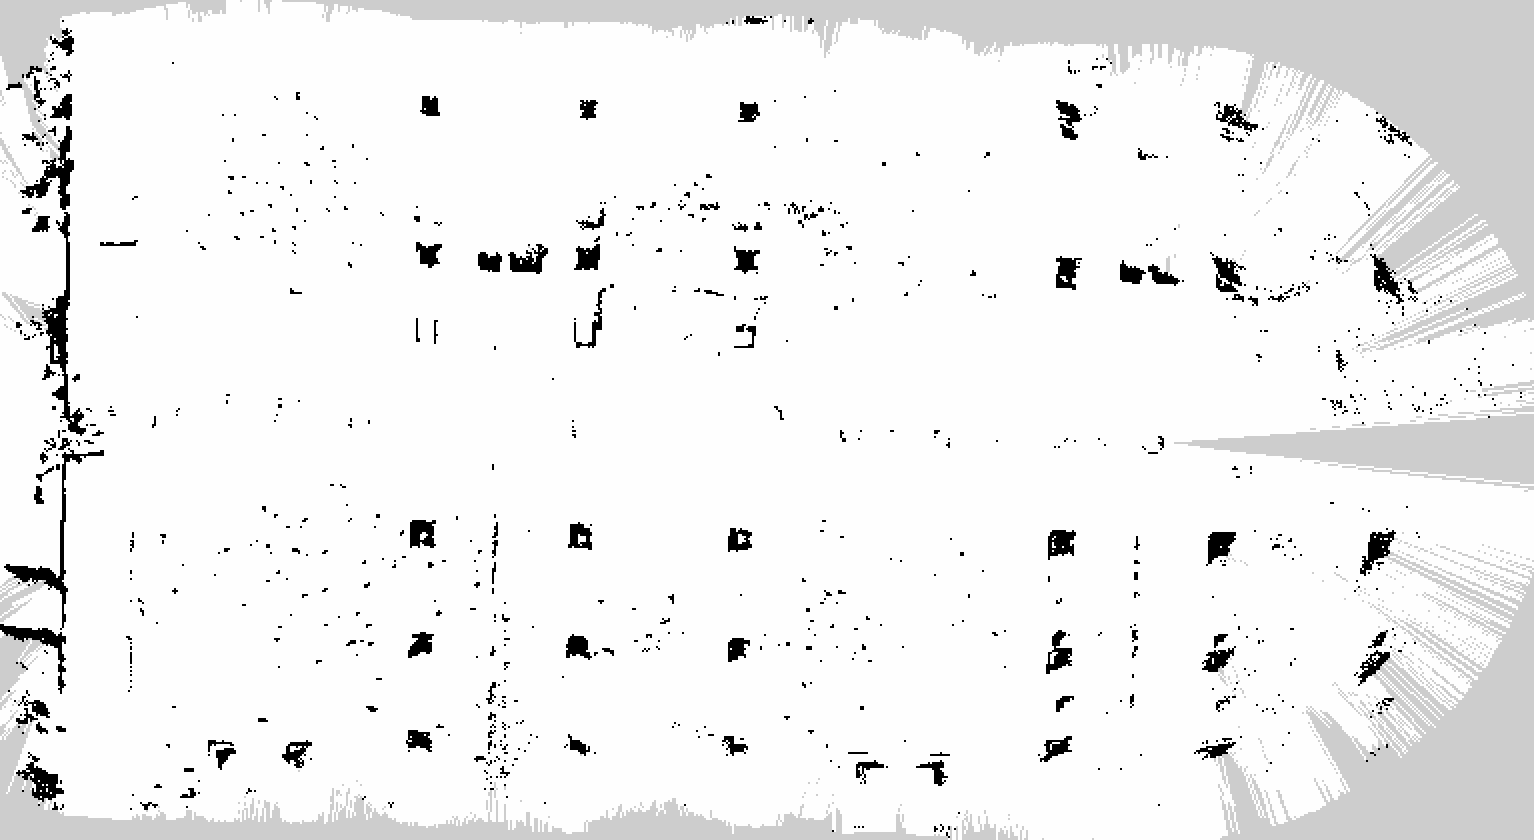
\includegraphics[width=0.8\textwidth]{gambar/bab4/pgm_gitet.png}
\caption{Peta Grid Titik (Point Grid Map) Hasil Pemetaan}
\label{fig:point_grid_map}
\footnotesize{\textbf{Sumber:} Dokumentasi Penulis}
\end{figure}

Namun, berdasarkan analisis terhadap hasil peta yang diperoleh, ditemukan bahwa peta tersebut tidak memiliki keragaman bentuk yang memadai untuk mendukung proses lokalisasi berbasis peta. Hal ini disebabkan oleh karakteristik struktur di gardu induk, seperti \textit{bracket} dan peralatan listrik lainnya, yang umumnya berukuran kecil, bersifat simetris, dan sulit terdeteksi secara konsisten dalam representasi dua dimensi. Akibatnya, sistem tidak mampu membentuk peta dengan fitur yang cukup kaya untuk mendukung lokalisasi yang akurat. Karena keterbatasan tersebut, sistem lokalisasi dalam penelitian ini tidak menggunakan pendekatan berbasis peta, melainkan mengandalkan metode odometri yang didukung oleh algoritma \textit{FastLIO2}. Posisi awal robot ditentukan secara tetap, dan proses lokalisasi dilakukan relatif terhadap posisi tersebut selama robot bergerak di lingkungan operasional. Sistem ini dapat dioptimalkan lebih lanjut melalui integrasi dengan sistem \textit{dock charging}, seperti yang digunakan pada robot Deep Robotics X30, untuk memastikan posisi awal robot selalu konsisten sebelum memulai aktivitas patroli. Pendekatan ini penting untuk mempertahankan ketepatan lokalisasi tanpa mengandalkan pemetaan global dalam lingkungan yang minim fitur visual.



\subsection{Pengujian Transmisi ke \emph{Control Station}}
Pengujian transmisi citra termal dari robot ke \emph{Control Station} dilakukan untuk memastikan bahwa sistem mampu mengirimkan data secara \emph{real-time}. Pengujian ini mencakup pengiriman data posisi, orientasi robot, dan status sensor menggunakan protokol \emph{WebSocket}, serta pengiriman citra termal, RGB, dan data akustik melalui protokol \emph{WebRTC}. Untuk mengevaluasi performa komunikasi, dilakukan pengujian pengiriman data secara kontinu dalam berbagai skenario, termasuk lingkungan dengan interferensi elektromagnetik dari peralatan gardu induk. Hasil pengujian menunjukkan bahwa sistem dapat mempertahankan komunikasi dengan latensi rata-rata sebesar 180–250 ms untuk data citra (video termal dan RGB), serta sekitar 30–50 ms untuk data posisi dan status sensor.

Meskipun terdapat potensi gangguan elektromagnetik di sekitar gardu, kualitas komunikasi tetap stabil berkat penggunaan antena eksternal berdaya tinggi pada robot dan \emph{Control Station}. Jarak pengujian antara robot dan \emph{Control Station} berkisar antara 80 hingga 100 meter, dan tidak ditemukan pemutusan koneksi selama pengujian berlangsung. Hasil pengujian menunjukkan bahwa sistem komunikasi telah mampu memenuhi kebutuhan transmisi data secara waktu nyata dalam skenario lapangan. Latensi transmisi data video yang berada di bawah 300 ms masih dapat diterima untuk aplikasi monitoring visual secara langsung. Sementara itu, latensi data posisi yang berada di bawah 100 ms cukup responsif untuk mendukung kebutuhan pemantauan posisi robot secara aktual.

Penggunaan protokol \emph{WebRTC} terbukti efektif dalam menangani transmisi video secara adaptif berdasarkan kualitas jaringan, sehingga mampu mengatasi fluktuasi bandwidth tanpa terjadi gangguan signifikan. Di sisi lain, \emph{WebSocket} memberikan keunggulan pada pengiriman data ringan seperti posisi dan status sensor karena overhead yang rendah dan komunikasi yang persisten.Secara keseluruhan, sistem transmisi ini telah menunjukkan kinerja yang dapat diandalkan untuk digunakan dalam aplikasi pengawasan jarak jauh di lingkungan gardu induk.


\subsection{\emph{Simulation Testing}}

Pengujian simulasi dilakukan dengan menggunakan data \emph{rosbag} yang diperoleh dari pengujian lapangan. Dalam simulasi ini, data dari \emph{rosbag} digunakan untuk merekonstruksi kondisi nyata, termasuk data LiDAR dan IMU untuk proses lokalisasi serta data citra dari kamera termal sebagai masukan deteksi suhu. Sistem kemudian diintegrasikan dengan antarmuka web, di mana jadwal patroli ditentukan sebelumnya. Saat robot tiba di titik inspeksi yang telah ditentukan, sistem akan melakukan analisis suhu pada posisi tersebut. Apabila terdeteksi adanya \emph{overheat}—yang pada simulasi ini disederhanakan menjadi suhu di atas 30\textdegree C—maka sistem akan mengirimkan data ke \emph{Web GUI} dan mencoba memprediksi posisi komponen yang mengalami anomali berdasarkan komponen terdekat pada peta.

Pengujian dilakukan sebanyak lima kali dengan konfigurasi \emph{waypoint}, jadwal patroli, dan ambang suhu yang berbeda. Adapun hasil pengujian adalah sebagai berikut \ref{tab:simulasi_overheat}


\begin{table}[H]
    \centering
    \caption{Hasil Pengujian Simulasi Deteksi \emph{Overheat}}
    \label{tab:simulasi_overheat}
    \begin{tabular}{|c|p{6cm}|p{5.5cm}|}
    \hline
    \textbf{No} & \textbf{Kondisi} & \textbf{Hasil} \\ \hline
    1 & Terdeteksi suhu di atas ambang, data komponen tersedia & Data dikirim ke web dan posisi komponen berhasil diprediksi dengan benar berdasarkan peta \\ \hline
    2 & Tidak ada suhu yang melewati ambang batas & Robot melakukan patroli hingga selesai tanpa mengirim data anomali \\ \hline
    3 & \emph{Overheat} terdeteksi, namun tidak ada data komponen pada titik deteksi & Sistem mengirim data dan menetapkan lokasi komponen sebagai titik deteksi \\ \hline
    4 & Semua proses berjalan baik: deteksi, prediksi posisi, dan pengiriman data & Sukses penuh, data komponen sesuai dengan prediksi lokasi \\ \hline
    5 & Deteksi gagal karena model tidak dapat mengenali objek pada citra & Sistem tidak dapat melanjutkan proses analisis dan data tidak terkirim \\ \hline
    \end{tabular}
    \end{table}

    Adapun hasil pengujian dimana robot mampu menetukan posisi komponen \emph{overheat}  berdasarkan data suhu yang terdeteksi, dapat dilihat pada diman apada pengujian ini ambang batas \emph{overheat} pada \emph{current transformator} diatur pada 40 C Gambar \ref{fig:simulasi_overheat}

    \begin{figure}[H]
    \centering
    \includegraphics[width=0.8\textwidth]{gambar/bab4/final.png}
    \caption{Hasil Simulasi Deteksi \emph{Overheat} pada Citra Termal}
    \label{fig:simulasi_overheat}
    \footnotesize{\textbf{Sumber:} Dokumentasi Penulis}
    \end{figure}

    Dimana dija dilakukan view secara detail pada komponen yang terdeteksi \emph{overheat} pada citra termal, seperti pada Gambar \ref{fig:simulasi_overheat_detail}.

    \begin{figure}[H]
        \centering
        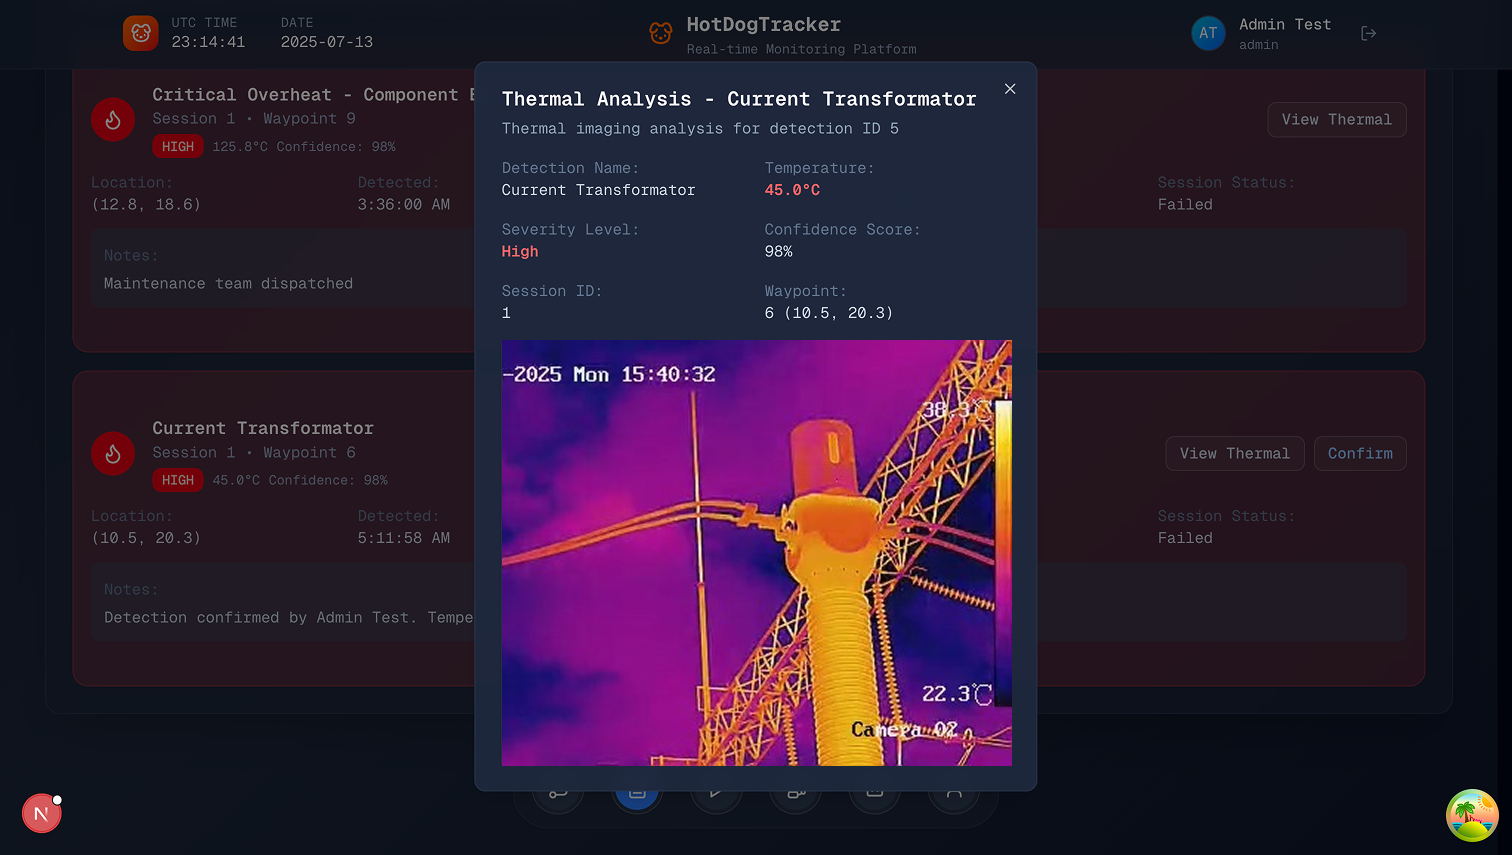
\includegraphics[width=0.8\textwidth]{gambar/bab4/webview.png}
        \caption{Hasil Simulasi Deteksi Detail \emph{Overheat} pada Citra Termal}
        \label{fig:simulasi_overheat_detail}
        \footnotesize{\textbf{Sumber:} Dokumentasi Penulis}
        \end{figure}
    

    Analisis hasil pengujian menunjukkan bahwa sistem mampu menjalankan deteksi dan prediksi komponen dengan baik ketika data termal dan basis data komponen tersedia secara konsisten. Kegagalan pada pengujian kelima menunjukkan bahwa keandalan model deteksi visual sangat mempengaruhi keberhasilan seluruh proses. Selain itu, ketiadaan data komponen (seperti pada pengujian ketiga) dapat diatasi dengan fallback lokasi, namun dengan risiko berkurangnya akurasi posisi. Oleh karena itu, kelengkapan basis data dan kualitas model deteksi menjadi dua aspek kritikal dalam keberhasilan sistem secara keseluruhan.


    \subsection{Hasil Pengujian \textit{Stress Test} WebSocket pada \textit{Frontend} (Next.js) dan \textit{Backend} (Express.js)}

    Pengujian stress test dilakukan untuk mengevaluasi ketahanan sistem end-to-end, mulai dari frontend berbasis Next.js hingga backend berbasis Express.js, terhadap aliran data intensif melalui protokol WebSocket. Dalam skenario ini, backend mengirimkan data secara kontinu ke klien setiap 0,02 detik (setara 50 pesan per detik), sementara frontend menerima, memproses, dan merender data secara real-time. Pengujian dijalankan menggunakan perangkat MacBook M4 dengan RAM 24 GB sebagai klien, dan VPS Biznet Neo dengan 4 vCPU dan 4 GB RAM sebagai server.
    
    Hasil pengujian menunjukkan bahwa sistem mampu menangani beban tinggi secara stabil. Di sisi frontend, kecepatan render rata-rata mencapai 61 FPS, dengan nilai minimum 57 FPS saat beban puncak, yang menunjukkan bahwa antarmuka tetap responsif dan halus. Latensi input tercatat stabil di kisaran 72 milidetik. Penggunaan CPU pada proses renderer berada pada rentang 38 hingga 45 persen, dan memori heap mencapai puncak sebesar 480 MB tanpa indikasi kebocoran memori. Di sisi backend, Express.js berhasil mengelola pengiriman data secara konsisten tanpa keterlambatan maupun kehilangan pesan, dengan waktu proses rata-rata per event di bawah 5 milidetik dan pemakaian CPU tetap di bawah 50 persen. Tidak ditemukan frame loss, dan antrean pesan WebSocket tetap terjaga di bawah 2 milidetik. Keberhasilan sistem dalam skenario ini didukung oleh optimasi arsitektur, seperti penggunaan web worker pada frontend untuk memproses data berat di luar main thread, penggunaan requestAnimationFrame untuk sinkronisasi rendering, serta penanganan asynchronous event yang efisien pada backend Express.js. Secara keseluruhan, sistem terbukti mampu menjalankan komunikasi dua arah berbasis WebSocket secara intensif tanpa penurunan performa yang berarti.
    